
% MORGAN STANLEY RESEARCH - LATEX STYLE GUIDE
% REFINED FOR VISUAL ACCURACY

\documentclass[10pt, a4paper]{article}
\usepackage[a4paper, top=2.2cm, bottom=2.5cm, left=1.4cm, right=1.4cm, headheight=1.5cm]{geometry}
\usepackage[T1]{fontenc}
\usepackage[scaled]{helvet}
\renewcommand{\familydefault}{\sfdefault}

\usepackage[table]{xcolor}
\usepackage{graphicx}
\usepackage{tcolorbox}
\usepackage{booktabs}
% \usepackage{colortbl} % Removed to prevent conflict
\usepackage{array}
\usepackage{tabularx}
\usepackage{fancyhdr}
\usepackage{tikz}
\usepackage{pgfplots}
\usepackage{float}
\usepackage{caption}
\usepackage{multicol}
\usepackage{adjustbox}
\usepackage{titlesec}
\usepackage{enumitem}
\usepackage{hyperref}

% Hyperref setup for clickable TOC
\hypersetup{
    colorlinks=true,
    linkcolor=msblue,
    urlcolor=msbrightblue,
    citecolor=msblue,
    pdftitle={Apple \& Intel Foundry: The Strategic Pivot},
    pdfauthor={Morgan Stanley Research},
}

% Fix for array/colortbl compatibility issue with p columns
\makeatletter
\let\insert@pcolumn\insert@column
\makeatother

% --- BRAND COLORS ---
\definecolor{msblue}{HTML}{002A5C}       % Morgan Stanley Dark Blue
\definecolor{msbrightblue}{HTML}{0096D6} % Light Blue for "INSIGHT" and Highlights
\definecolor{msgrey}{HTML}{F2F2F2}       % Light Grey for Backgrounds
\definecolor{mstextgrey}{HTML}{666666}   % Grey text for analysts
\definecolor{mstableheader}{HTML}{E5E5E5} % Grey for table headers

% --- PAGE HEADER/FOOTER ---
\pagestyle{fancy}
\fancyhf{}
\renewcommand{\headrulewidth}{0pt}

% Left Header: Logo
\lhead{
    \vspace{0.2cm}
    {\fontsize{14}{14}\bfseries Morgan Stanley} 
    \hspace{0.15cm} \textcolor{black}{|} \hspace{0.15cm} 
    {\footnotesize\bfseries RESEARCH} \\
    {\color{mstextgrey}\footnotesize \today}
}

% Right Header: Region/Type
\rhead{
    \vspace{0.2cm}
    {\color{msbrightblue}\bfseries\small ASIA PACIFIC INSIGHT} % Dynamic based on region
}

% Footer
\lfoot{\color{mstextgrey}\footnotesize Morgan Stanley Research}
\rfoot{\bfseries\thepage}

% --- TYPOGRAPHY & SECTIONS ---
\titleformat{\section}
  {\color{msblue}\normalfont\Large\bfseries}{}{0em}{}
  
\titleformat{\subsection}
  {\color{black}\normalfont\large\bfseries}{}{0em}{}

% --- CUSTOM COMMANDS ---

% 1. Report Title Block
\newcommand{\reporttitle}[3]{%
    \vspace{0.5cm}
    {\fontsize{14}{16}\selectfont\color{msbrightblue}\bfseries #1 \par} % Ticker/Company
    \vspace{0.1cm}
    {\fontsize{28}{32}\selectfont\color{black}\fontseries{l}\selectfont #2 \par} % Main Title
    \vspace{0.5cm}
}

% 2. "What's Changed" / Estimates Table
\newcommand{\estimatesbox}[1]{%
    \begin{tcolorbox}[colback=msgrey, colframe=white, boxrule=0pt, sharp corners, left=2pt, right=2pt, top=2pt, bottom=2pt]
    \textbf{\footnotesize WHAT'S CHANGED}
    \end{tcolorbox}
    \vspace{-0.3cm}
    #1
    \vspace{0.5cm}
}

% 3. Sidebar Analyst Info
\newcommand{\analystinfo}[3]{%
    {\bfseries\small #1} \\
    {\color{mstextgrey}\tiny #2} \\
    {\color{mstextgrey}\tiny #3} \\
    \vspace{0.2cm}
}

% 4. Stock Rating Box
\newcommand{\ratingbox}[3]{%
    \begin{tcolorbox}[colback=msgrey, colframe=msgrey, sharp corners, boxrule=0pt]
    \textbf{\small #1} \\ % Company Name
    \scriptsize #2 \\      % Industry
    \vspace{0.1cm}
    \textbf{\large #3}      % Rating (Overweight)
    \end{tcolorbox}
}

% 5. Blue Section Header (The "Morgan Stanley" Section Divider)
\newcommand{\blueheader}[1]{%
    \vspace{0.5cm}
    {\color{msblue}\bfseries\large #1}
    \par\vspace{0.1cm}
}

% --- GLOBAL TABLE RULE ---
\newcommand{\tablefont}{\footnotesize} % Global font size for tables

% --- CONSISTENT TABLE FORMATTING ---
% Use this environment for all tables to ensure consistent font sizes
% even when using adjustbox for width control
\newenvironment{mstable}[1][\textwidth]{%
    \tablefont%
    \renewcommand{\arraystretch}{1.2}%
    \rowcolors{2}{msgrey}{white}%
    \begin{adjustbox}{max width=#1, center}%
}{%
    \end{adjustbox}%
}

% Alternative: For tables that MUST fit but should not shrink font below \scriptsize
\newenvironment{mstablescaled}[1][\textwidth]{%
    \scriptsize% Minimum readable font size
    \renewcommand{\arraystretch}{1.3}%
    \rowcolors{2}{msgrey}{white}%
    \begin{adjustbox}{max width=#1, center}%
}{%
    \end{adjustbox}%
}

% --- CHART STYLES ---
\pgfplotsset{
    compat=1.18,
    width=\linewidth, % Responsive width
    height=6cm,
    % Define RdYlGn colormap (Red-Yellow-Green)
    colormap={RdYlGn}{rgb255(0cm)=(215,48,39); rgb255(0.25cm)=(253,174,97); rgb255(0.5cm)=(255,255,191); rgb255(0.75cm)=(166,217,106); rgb255(1cm)=(26,152,80)},
    % Custom cycle list for multi-series bar charts
    cycle list={
        {fill=msblue},
        {fill=msbrightblue},
        {fill=gray},
        {fill=msblue!40},
    },
    % GLOBAL FIX: Use pgfplots' built-in area legend style for all ybar charts
    % This ensures proper vertical alignment with text using font-relative units
    /pgfplots/ybar legend/.style={
        area legend,
    },
    % STANDARD LEGEND POSITIONING: Below chart, centered, horizontal layout
    mslegend/.style={
        legend style={at={(0.5,-0.15)}, anchor=north, legend columns=-1, draw=none, font=\footnotesize}
    },
    % Default legend style for all charts (can be overridden per chart)
    every axis/.append style={
        legend style={at={(0.5,-0.15)}, anchor=north, legend columns=-1, draw=none, font=\footnotesize}
    },
    msstyle/.style={
        ybar,
        fill=msblue,
        bar width=15pt,
        draw=none,
        axis line style={draw=none},
        tick style={draw=none},
        ymajorgrids=true,
        grid style={dotted, gray},
        nodes near coords,
        nodes near coords style={font=\tiny, color=black},
        axis x line*=bottom,
        x axis line style={draw=gray},
    },
    % Specific style for small-data charts to prevent wide bars
    compactchart/.style={
        msstyle,
        width=0.5\textwidth,
        enlarge x limits=0.5,
    },
    % Color-coded bar chart style
    colorbar/.style={
        ybar,
        bar width=30pt,
        draw=none,
        axis line style={draw=gray},
        tick style={draw=none},
        ymajorgrids=true,
        grid style={dotted, gray},
        nodes near coords,
        nodes near coords align={vertical},
        nodes near coords style={font=\bfseries\footnotesize, color=black},
        axis x line*=bottom,
        axis y line*=left,
    },
    % SEMANTIC CHART STYLES - Use these for consistent coloring
    % For diverging data (bad to good: red-yellow-green)
    divergingstyle/.style={
        ybar,
        bar width=30pt,
        draw=none,
        axis line style={draw=gray},
        tick style={draw=none},
        ymajorgrids=true,
        grid style={dashed, gray},
        nodes near coords,
        nodes near coords align={vertical},
        nodes near coords style={font=\bfseries\footnotesize, color=black},
        axis x line*=bottom,
        axis y line*=left,
    },
    % For company comparisons (TSMC/Intel/Samsung) with visual distinction
    comparestyle/.style={
        ybar,
        bar width=30pt,
        draw=none,
        axis line style={draw=none},
        tick style={draw=none},
        ymajorgrids=true,
        grid style={dotted, gray},
        nodes near coords,
        nodes near coords align={vertical},
        nodes near coords style={font=\footnotesize},
        axis x line*=bottom,
        enlarge x limits=0.3,
    }
}

\begin{document}
\reporttitle{Apple Inc. (AAPL) \& Intel Corp. (INTC)}{Apple \& Intel Foundry: The Strategic Pivot -- Analyzing the 14A/18A Bifurcation Rumors}{}

\begin{tcolorbox}[colback=msgrey, colframe=white, boxrule=0pt, sharp corners, left=2pt, right=2pt, top=2pt, bottom=2pt]
\begin{minipage}{0.65\textwidth}
    \textbf{\footnotesize ANALYST CERTIFICATION AND IMPORTANT DISCLOSURES ARE LISTED IN THE APPENDIX.}
\end{minipage}
\hfill
\begin{minipage}{0.3\textwidth}
    \raggedleft \tiny \textbf{Stock Ratings} \\
    \textbf{AAPL: OVERWEIGHT} \\
    \textbf{INTC: EQUAL-WEIGHT}
\end{minipage}
\end{tcolorbox}
\vspace{0.5cm}

% --- TABLE OF CONTENTS PAGE ---
\newpage
\thispagestyle{fancy}

% TOC Header with Morgan Stanley Styling
\begin{tcolorbox}[
    colback=white, 
    colframe=msblue, 
    boxrule=2pt, 
    arc=0pt, 
    outer arc=0pt,
    left=15pt, 
    right=15pt, 
    top=12pt, 
    bottom=12pt,
    width=\textwidth
]
{\color{msblue}\fontsize{22}{26}\selectfont\bfseries Table of Contents}
\vspace{0.1cm}

{\color{mstextgrey}\footnotesize Apple Inc. (AAPL) \& Intel Corp. (INTC) --- Strategic Analysis Report}
\end{tcolorbox}

\vspace{0.5cm}

% Custom TOC styling for consistent appearance
\makeatletter
% Style for section entries
\renewcommand*\l@section[2]{%
    \ifnum \c@tocdepth >\z@
    \addpenalty\@secpenalty
    \addvspace{1.0em \@plus\p@}%
    \setlength\@tempdima{2.5em}%
    \begingroup
        \parindent \z@ \rightskip \@pnumwidth
        \parfillskip -\@pnumwidth
        \leavevmode \color{msblue}\bfseries
        \advance\leftskip\@tempdima
        \hskip -\leftskip
        #1\nobreak\hfil \nobreak\hb@xt@\@pnumwidth{\hss \color{black}#2}\par
    \endgroup
    \fi}

% Style for subsection entries  
\renewcommand*\l@subsection[2]{%
    \ifnum \c@tocdepth >\@ne
    \addpenalty\@secpenalty
    \addvspace{0.3em \@plus\p@}%
    \setlength\@tempdima{3.5em}%
    \begingroup
        \parindent \z@ \rightskip \@pnumwidth
        \parfillskip -\@pnumwidth
        \leavevmode \footnotesize
        \advance\leftskip\@tempdima
        \hskip -\leftskip
        #1\nobreak\leaders\hbox{$\m@th
            \mkern \@dotsep mu\hbox{.}\mkern \@dotsep
            mu$}\hfil \nobreak\hb@xt@\@pnumwidth{\hss #2}\par
    \endgroup
    \fi}
\makeatother

% Set TOC depth to show sections and subsections
\setcounter{tocdepth}{2}

% Render TOC with custom formatting
\begin{tcolorbox}[
    colback=msgrey, 
    colframe=white, 
    boxrule=0pt, 
    arc=0pt,
    left=15pt, 
    right=15pt, 
    top=15pt, 
    bottom=15pt,
    width=\textwidth
]
\renewcommand{\contentsname}{}
{\hypersetup{linkcolor=black}
\makeatletter
\@starttoc{toc}
\makeatother}
\end{tcolorbox}

\vspace{0.3cm}

% Key Sections Quick Reference
\begin{tcolorbox}[
    colback=white, 
    colframe=msbrightblue, 
    boxrule=1pt, 
    arc=0pt,
    left=12pt, 
    right=12pt, 
    top=10pt, 
    bottom=10pt,
    title={\color{white}\bfseries\footnotesize KEY SECTIONS AT A GLANCE},
    colbacktitle=msbrightblue,
    coltitle=white
]
\footnotesize
\begin{tabular}{@{}p{0.45\textwidth}p{0.45\textwidth}@{}}
\textbf{\color{msblue}Section 1:} The Rumor Mill \& Strategic Rationale & \textbf{\color{msblue}Section 4:} Valuation Models \\[0.2cm]
\textbf{\color{msblue}Section 2:} IFS Assessment: 18A/14A Readiness & \textbf{\color{msblue}Section 5:} Investment Risks \\[0.2cm]
\textbf{\color{msblue}Section 3:} Technological Deep Dive & \\
\end{tabular}
\end{tcolorbox}

\newpage

\begin{multicols}{2}

\ratingbox{Apple Inc. (AAPL)}{Technology Hardware}{OVERWEIGHT}
\vspace{0.2cm}


\estimatesbox{
\begin{itemize}[leftmargin=*]
    \item \textbf{Intel 18A Timeline:} Risk production commenced Q2 2025; rumors suggest Apple low-end M-series adoption by mid-2027.
    \item \textbf{Yield Considerations:} Recent reports indicate 18A yields near $\sim$10\% (Summer 2025); viability threshold for Apple is $>$70\%.
    \item \textbf{Foundry Financials:} IFS operating losses peaked at $\sim$\$13B in 2024; break-even target remains $\sim$2027.
\end{itemize}
}



\textbf{The Conditional Validation: A Strategic Bifurcation, Not a Pivot}

The semiconductor landscape is buzzing with reports that Apple is exploring Intel Foundry Services (IFS) for its future silicon needs. Specifically, rumors suggest Apple may utilize Intel's \textbf{18A process node} for entry-level M-series chips (MacBook Air, iPad) starting roughly \textbf{mid-2027}, with speculative long-range roadmaps hinting at the \textbf{14A node} for non-Pro iPhone chips by \textbf{2028}.

We view this development not as a wholesale abandonment of TSMC, but as a \textbf{"Conditional Validation"} of Intel's IDM 2.0 strategy. It represents a calculated \textbf{Tiered Adoption} strategy by Apple: bifurcating its supply chain to mitigate geopolitical risk while maintaining performance leadership through TSMC for its flagship products.

\textbf{1. The Tiered Adoption Strategy: High-Volume vs. High-Performance}
Our analysis of the supply chain suggests Apple is constructing a "Second Source" architecture. The bifurcation logic is clear:
\begin{itemize}
    \item \textbf{Intel 18A (The Resilience Tier):} Designated for \textbf{lower-margin, high-volume devices} like the MacBook Air and iPad Air. These products are less sensitive to the absolute peak of performance-per-watt metrics compared to the iPhone Pro series but require massive volume (estimated \textbf{15--20 million units/year}). Utilizing Intel here allows Apple to "test run" the foundry without risking its crown jewels.
    \item \textbf{TSMC N2/A16 (The Performance Tier):} We expect Apple to retain TSMC as the exclusive partner for "Pro" tier silicon (M-Max/Ultra, iPhone Pro A-series). TSMC's proven yield consistency and upcoming \textbf{N2 (2nm)} and \textbf{A16 (1.6nm)} nodes offer the predictable performance scaling required for flagship differentiation.
\end{itemize}

\textbf{2. Key Catalysts: Why Now?}
Three converging forces are driving this strategic pivot:
\begin{enumerate}
    \item \textbf{Geopolitical "Insurance":} With rising tensions in the Taiwan Strait, Apple is under increasing pressure to align with the "Made in USA" mandate. Intel's Arizona and Ohio fabs, backed by \textbf{\$7.86 billion in direct CHIPS Act funding}, offer the only viable domestic alternative for sub-2nm logic.
    \item \textbf{TSMC Capacity Constraints:} TSMC's advanced nodes are heavily subscribed by NVIDIA and AMD for AI accelerators. Offloading "commodity" Apple Silicon to Intel relieves pressure on TSMC's capacity, potentially freeing up wafers for higher-margin AI chips.
    \item \textbf{Technological Convergence:} Intel's aggressive roadmap---introducing \textbf{RibbonFET} (Gate-All-Around) and \textbf{PowerVia} (Backside Power Delivery) with 18A---technically leapfrogs TSMC's N2 in specific power-delivery metrics. If executed, 18A offers a credible alternative for mobile efficiency.
\end{enumerate}

\textbf{3. Financial Implications: The \$13 Billion Question}
For Intel, securing Apple is existential. IFS reported \textbf{operating losses exceeding \$13 billion in 2024}. An Apple contract provides the baseload volume necessary to fill the new mega-fabs and amortize the massive CapEx associated with High-NA EUV integration. Without a "Hero Customer" like Apple, Intel's path to break-even operating margins by \textbf{2027} remains perilous.

For Apple, this move creates leverage. By establishing a viable second source, Apple erodes TSMC's pricing monopoly (currently holding $\sim$90\% of the 3nm market), potentially negotiating better terms for its N2/A16 wafers.

\textbf{Verdict: A Probationary Partnership}
While the strategic rationale is sound, execution risk remains the dominant variable. With 18A yields reportedly struggling at $\sim$10\% in mid-2025, Intel has a massive gap to close to meet Apple's $>$70\% commercial viability standard. We classify this potential partnership as \textbf{probationary}: Apple has engaged, but full production remains contingent on Intel proving it can deliver yield, volume, and performance stability by Q1 2026.

\vspace{0.5cm}

\begin{center}
\captionof{table}{Rumored Apple-Intel Roadmap vs. TSMC Baseline}
\rowcolors{2}{msgrey}{white}
\tablefont
\begin{tabular}{p{0.22\columnwidth}p{0.22\columnwidth}p{0.22\columnwidth}p{0.22\columnwidth}}
\toprule
\textbf{Feature} & \textbf{Intel 18A (Rumored)} & \textbf{TSMC N2 (Baseline)} & \textbf{Intel 14A (Speculative)} \\
\midrule
\textbf{Target Product} & MacBook Air / iPad & iPhone Pro / M-Pro & iPhone (Non-Pro) \\
\textbf{Production Start} & H2 2025 (Risk) & H2 2025 (Vol) & 2027 (Risk) \\
\textbf{Apple Launch} & Mid-2027 & Late 2025 (N3)/2026 & 2028 \\
\textbf{Key Tech} & RibbonFET + PowerVia & GAA Nanosheet & High-NA EUV \\
\textbf{Yield Status} & $\sim$10\% (Low Maturity) & Proven HVM & In Development \\
\textbf{Primary Driver} & Supply Chain Resilience & Performance Leadership & Cost/Density \\
\bottomrule
\end{tabular}
\par\vspace{0.1cm}
{\tiny Source: Industry Reports, Morgan Stanley Research Estimates}
\end{center}

\vspace{0.5cm}

\begin{center}
\captionof{figure}{Intel Foundry Services: The Path to Break-Even (Operating Loss in \$B)}
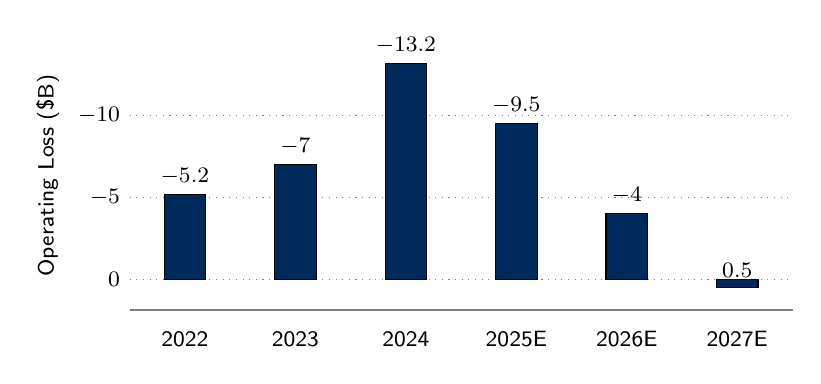
\begin{tikzpicture}
\begin{axis}[
    msstyle,
    width=10cm,
    symbolic x coords={2022, 2023, 2024, 2025E, 2026E, 2027E},
    xtick=data,
    xticklabel style={font=\footnotesize},
    nodes near coords={\pgfmathprintnumber\pgfplotspointmeta},
    nodes near coords style={font=\footnotesize, color=black, anchor=south},
    ylabel={Operating Loss (\$B)},
    ylabel style={font=\footnotesize},
    yticklabel style={font=\footnotesize},
    y dir=reverse,
    axis lines*=left,
    ymajorgrids=true,
    height=5cm,
    bar width=15pt
]
\addplot[fill=msblue] coordinates {(2022,-5.2) (2023,-7.0) (2024,-13.2) (2025E,-9.5) (2026E,-4.0) (2027E,0.5)};
\end{axis}
\pgfplotsset{
    after end axis/.append code={
        \node[anchor=north, font=\tiny, text width=10cm, align=center] at (current axis.south) [yshift=-1cm] {
            Source: Company Data, Morgan Stanley Research Estimates (2025-2027E)
        };
    }
}
\end{tikzpicture}
\end{center}

\end{multicols}

The rumored bifurcation of Apple's silicon supply chain---retaining TSMC for flagship processors while qualifying Intel Foundry Services (IFS) for entry-level M-series chips---represents the most significant structural shift in Apple's semiconductor strategy since the transition from Intel x86 to Apple Silicon. This move is less about immediate performance arbitrage and more about \textbf{geopolitical resilience} and \textbf{supply chain leverage}. Our analysis suggests that while Intel's 18A node offers theoretical technological parity with TSMC's N2, the decision is driven by Apple's need to hedge against Taiwan Strait concentration risk and to align with U.S. industrial policy.

\subsection*{The Geopolitical Imperative: De-Risking the \$3 Trillion Ecosystem}
Apple's reliance on TSMC is absolute; currently, nearly 100\% of Apple's advanced logic (A-series, M-series) is manufactured in Taiwan. This creates a single point of failure for a company with a market capitalization exceeding \$3 trillion.
\begin{itemize}
    \item \textbf{The "Made in USA" Mandate:} With the U.S. CHIPS Act allocating \textbf{\$7.86 billion in direct funding} and up to \textbf{\$11 billion in loans} to Intel, the political pressure for Apple to support a domestic champion is intensifying. Apple has already pledged \textbf{\$430 billion} (later updated to over \textbf{\$600 billion}) in U.S. investments; sourcing wafers from Intel's Arizona and Ohio fabs is the logical next step in this commitment.
    \item \textbf{Supply Chain Resilience:} The "China+1" strategy, which has seen Apple shift assembly to India and Vietnam, is now moving upstream to wafer fabrication. Intel provides the only sub-2nm capacity outside of East Asia. While TSMC's Arizona fabs are coming online, they face higher costs (estimated at \textbf{30--50\% higher than Taiwan}) and rely on the same Taiwanese IP backbone. A distinct "Second Source" with Intel diversifies the \textit{foundry risk}, not just the geographic risk.
\end{itemize}

\subsection*{The "Test Run" Configuration: M-Series as the Trojan Horse}
Reports indicate Apple is eyeing the \textbf{Intel 18A node} specifically for "entry-level" M-series chips (e.g., MacBook Air, iPad Air) by \textbf{mid-2027}. This targeting is strategic and deliberate, minimizing execution risk while establishing a foothold.
\begin{itemize}
    \item \textbf{Volume Alignment:} The entry-level Mac/iPad segment represents roughly \textbf{15--20 million units annually}. This volume is substantial enough to be meaningful for Intel's fab utilization but small enough to be manageable if yield ramps are slower than anticipated. It avoids the "all-in" risk of shifting the iPhone (200M+ units), where a yield failure would be catastrophic.
    \item \textbf{Performance Sensitivity:} While the iPhone's thermal envelope is unforgiving, the MacBook Air and iPad Air have slightly more relaxed constraints. This makes them ideal candidates for qualifying a new process node like 18A, which introduces radical new transistor architectures (\textbf{RibbonFET}) that may require multiple iterations to perfect.
\end{itemize}

\begin{center}
\captionof{figure}{Global Advanced Node Manufacturing Capacity Share (2024 vs. 2030E)}
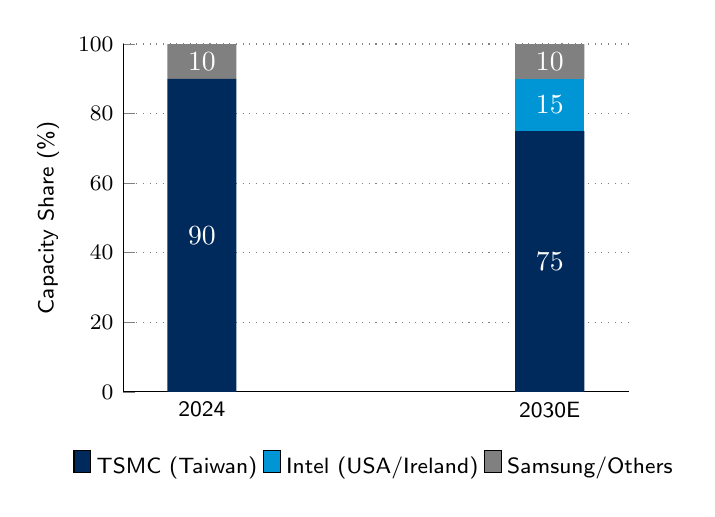
\begin{tikzpicture}
\begin{axis}[
    ybar stacked,
    height=6cm,
    width=8cm,
    bar width=25pt,
    enlarge x limits={abs=1cm},
    legend style={at={(0.5,-0.15)}, anchor=north, legend columns=-1, draw=none, font=\footnotesize},
    ylabel={Capacity Share (\%)},
    ylabel style={font=\footnotesize},
    symbolic x coords={2024, 2030E},
    xtick=data,
    xticklabel style={font=\footnotesize},
    ymin=0, ymax=100,
    axis y line*=left,
    axis x line*=bottom,
    ymajorgrids=true,
    grid style={dotted, gray},
    nodes near coords,
    nodes near coords style={font=\footnotesize, color=white, font=\bfseries},
    every node near coord/.append style={
        anchor=center
    },
    yticklabel style={font=\footnotesize},
    title style={at={(0.5,-0.4)}, anchor=north, font=\tiny, text width=8cm, align=center},
    cycle list={
        {fill=msblue, draw=none},
        {fill=msbrightblue, draw=none},
        {fill=gray, draw=none},
    }
]
\addplot coordinates {(2024,90) (2030E,75)}; % TSMC
\addlegendentry{TSMC (Taiwan)}
\addplot coordinates {(2024,0) (2030E,15)}; % Intel Foundry  
\addlegendentry{Intel (USA/Ireland)}
\addplot coordinates {(2024,10) (2030E,10)}; % Samsung/Others
\addlegendentry{Samsung/Others}
\end{axis}
\pgfplotsset{
    after end axis/.append code={
        \node[anchor=north, font=\tiny, text width=8cm, align=center] at (current axis.south) [yshift=-1.5cm] {
            Note: 2030E assumes successful Intel 18A/14A ramp and Apple adoption.\\
            Source: Morgan Stanley Research Estimates
        };
    }
}
\end{tikzpicture}
\end{center}

\subsection*{The Execution Gap: RibbonFET Reality vs. Yield Aspirations}
While the strategic logic is sound, the operational reality of Intel Foundry Services (IFS) remains the primary bottleneck. The transition to 18A is not merely a shrink; it involves the simultaneous introduction of two paradigm-shifting technologies: \textbf{RibbonFET} (Gate-All-Around transistors) and \textbf{PowerVia} (Backside Power Delivery).
\begin{itemize}
    \item \textbf{The 10\% Yield Crisis:} Recent channel checks suggest that early 18A test wafers in Summer 2025 were yielding near \textbf{10\%}. For a commercial foundry engagement, Apple typically demands yields exceeding \textbf{70--80\%} to ensure margin preservation. The gap between 10\% and 70\% represents a "Valley of Death" that Intel must cross in less than 18 months to meet the Q1 2026 PDK deadline.
    \item \textbf{Financial Bleed:} IFS operating losses peaked at over \textbf{\$13 billion in 2024}. While these losses are expected to narrow, the division is burning cash at a rate that necessitates external capital or massive customer prepayments. An Apple deal acts as a validator, but it cannot fund the CapEx alone; Intel must demonstrate it can manufacture 18A profitably, or risk becoming a subsidized entity dependent on government funds.
\end{itemize}

\subsection*{Strategic Verdict: A Hedge, Not a Replacement}
We reiterate our view that this potential partnership is a \textbf{hedge}. Apple is unlikely to abandon TSMC's N2 or A16 nodes for its premium silicon. TSMC's ecosystem---specifically its advanced packaging leadership with \textbf{CoWoS} and \textbf{SoIC}---is integral to the performance of the M-Max and M-Ultra chips. Intel's competitive packaging solutions (\textbf{EMIB}, \textbf{Foveros Direct}) are capable, but migrating Apple's complex custom designs from TSMC's PDK to Intel's PDK is a non-trivial engineering challenge that introduces significant "friction costs."

Therefore, we view the 2027-2028 timeframe as a "probationary period" where Intel serves as a secondary supplier for non-critical silicon, creating price competition for TSMC while establishing a U.S. supply baseload.

\vspace{0.5cm}

\begin{center}
\captionof{table}{Risk Assessment: Apple Adopting Intel 18A}
\rowcolors{2}{msgrey}{white}
\tablefont
\begin{tabular}{p{0.15\linewidth}p{0.35\linewidth}p{0.35\linewidth}c}
\toprule
\textbf{Risk Factor} & \textbf{Bull Case (Strategic Win)} & \textbf{Bear Case (Execution Failure)} & \textbf{Impact} \\
\midrule
\textbf{Process Yield} & Intel hits $>$70\% yield by 2026; 18A matches N2 performance. & Yields stall at 40-50\%; delays force Apple to revert to TSMC N3P/N2. & \cellcolor{red!20}Critical \\
\textbf{Cost Structure} & CHIPS Act \& 25\% ITC offset higher US labor/utility costs. & US wafer costs remain 30-50\% higher than Taiwan; dilutes Apple margins. & \cellcolor{orange!20}High \\
\textbf{Packaging} & Foveros Direct proves superior for 3D stacking (M-series). & Incompatibility with Apple's existing CoWoS designs forces redesigns. & \cellcolor{yellow!20}Medium \\
\textbf{Capacity} & Intel Arizona/Ohio fabs ramp on time (2025/2026). & Construction delays push volume availability to 2028+. & \cellcolor{orange!20}High \\
\bottomrule
\end{tabular}
\par\vspace{0.1cm}
{\tiny Source: Industry Data, Morgan Stanley Research Analysis}
\end{center}
\section{The Rumor Mill \& Strategic Rationale}

The prospect of Apple diverging from its exclusive partnership with TSMC represents the most significant potential disruption to the semiconductor supply chain in a decade. While Apple has historically championed a dual-source strategy (notably splitting the A9 chip between Samsung and TSMC in 2015), the company has spent the last eight years consolidating its advanced logic manufacturing solely with TSMC. The emerging rumors of a pivot to Intel Foundry Services (IFS) suggest a calculated strategic inflection point, driven not by immediate technical superiority, but by a complex matrix of geopolitical risk management, supply chain resilience, and commercial leverage.

\subsection{Analyst Consensus: The 18A vs. 14A Bifurcation}
Current intelligence indicates a bifurcated adoption strategy that aligns specific Intel process nodes with Apple's tiered product lines. The rumor mill, primarily driven by supply chain analysts Ming-Chi Kuo and Jeff Pu, points to a "crawl, walk, run" adoption curve rather than an abrupt switch.

\begin{itemize}
    \item \textbf{The M-Series Pilot (Intel 18A):} Ming-Chi Kuo reports that Apple is preparing to qualify Intel's \textbf{18A process} (and its performance variant 18A-P) for \textbf{entry-level M-series processors}---likely destined for the MacBook Air and iPad Air. The timeline targets a \textbf{mid-2027} launch, implying risk production must stabilize by early 2026. This aligns with Intel's 18A roadmap, which entered risk production in April 2025.
    \item \textbf{The iPhone Expansion (Intel 14A):} A more aggressive, albeit speculative, claim from Jeff Pu (Haitong International) suggests Apple could utilize Intel's successor node, \textbf{14A}, for \textbf{"non-Pro" iPhone silicon} (e.g., the A22 chip for iPhone 20/20e) by \textbf{2028}. This node introduces High-NA EUV lithography and second-generation RibbonFETs, theoretically offering the transistor density required for mobile SoCs.
\end{itemize}

This bifurcation---using a mature-by-then 18A for larger, lower-margin devices and reserving the cutting-edge 14A for high-volume mobile chips---mirrors Apple's previous bifurcation of the A-series chips (using older chips in non-Pro iPhones).

\begin{center}
\captionof{table}{Rumor Matrix: Apple's Potential Roadmap with Intel Foundry}
\rowcolors{2}{msgrey}{white}
\tablefont
\begin{tabular}{p{0.2\linewidth}p{0.15\linewidth}p{0.25\linewidth}p{0.3\linewidth}}
\toprule
\textbf{Analyst / Source} & \textbf{Target Node} & \textbf{Product Scope} & \textbf{Strategic Context \& Risk} \\
\midrule
\textbf{Ming-Chi Kuo} (TF Intl.) & Intel 18A / 18A-P & \textbf{MacBook Air / iPad} (Low-end M-Series) & \textbf{The "Pilot" Program:} Target volume of 15--20M units allows Apple to validate Intel's PDK without risking the flagship iPhone. Timeline: H2 2027. \\
\textbf{Jeff Pu} (Haitong / GF) & Intel 14A & \textbf{iPhone 20 / 20e} (Non-Pro A22) & \textbf{The "Volume" Play:} Contingent on 14A success. Would require Intel to master High-NA EUV cost-effectively. Timeline: 2028. \\
\textbf{Mark Gurman} (Bloomberg) & Strategic Inv. & \textbf{N/A} (Corporate Level) & Reported "deepened cooperation" and strategic talks in late 2025, validating the seriousness of the engagement beyond mere testing. \\
\bottomrule
\end{tabular}
\par\vspace{0.1cm}
{\tiny Source: Analyst Reports (Kuo, Pu, Gurman), Morgan Stanley Research Compilation}
\end{center}

\subsection{The "Low-Risk Test Run": Anatomy of a 15-Million Unit Bet}
The most credible scenario is the "Low-Risk Test Run" using the M-series. Apple ships approximately \textbf{200--230 million iPhones} annually, compared to roughly \textbf{20--25 million Macs}. Shifting the entire iPhone volume to an unproven foundry would be suicidal. However, shifting the \textbf{MacBook Air} volume (estimated at 15--20 million units) offers a perfect asymmetry of risk and reward:

\begin{enumerate}
    \item \textbf{Containment of Failure:} If Intel 18A yields are poor (currently rumored around \textbf{10\%} in early runs vs. the requisite 70\%+), the financial damage is limited to a lower-volume, lower-margin SKU. Apple could ostensibly backfill this supply with previous-generation chips from TSMC if necessary.
    \item \textbf{Capacity Utilization for Intel:} For Intel, 15 million wafers is a lifeline. With IFS reporting operating losses exceeding \textbf{\$13 billion in 2024}, filling the massive Ohio and Arizona fabs is an existential necessity. An Apple commitment, even for a "test run," validates the process for other potential customers like NVIDIA or Qualcomm.
    \item \textbf{Thermal Latitude:} The MacBook Air chassis, while fanless, has a larger thermal mass than an iPhone. It can tolerate slightly higher power leakage or lower efficiency curves that might occur in the early stages of a new process node (like 18A's PowerVia implementation) better than a battery-constrained smartphone.
\end{enumerate}

\begin{center}
\captionof{figure}{The "Test Run" Scale: Potential Intel Volume vs. Total Apple Demand (2027E)}
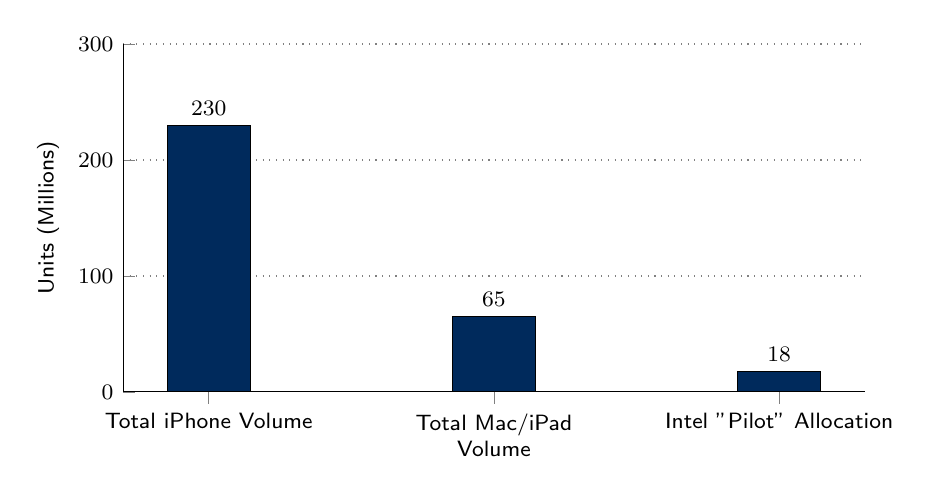
\begin{tikzpicture}
\begin{axis}[
    ybar,
    width=11cm,
    height=6cm,
    symbolic x coords={Total iPhone Volume, Total Mac/iPad Volume, Intel "Pilot" Allocation},
    xtick=data,
    xticklabel style={font=\footnotesize, text width=3cm, align=center},
    nodes near coords,
    nodes near coords align={vertical},
    nodes near coords style={font=\footnotesize},
    ymin=0, ymax=300,
    ylabel={Units (Millions)},
    ylabel style={font=\footnotesize},
    yticklabel style={font=\footnotesize},
    axis y line*=left,
    axis x line*=bottom,
    ymajorgrids=true,
    grid style={dotted, gray},
    bar width=30pt,
    enlarge x limits=0.15
]
\addplot[fill=msblue] coordinates {(Total iPhone Volume, 230) (Total Mac/iPad Volume, 65) (Intel "Pilot" Allocation, 18)};
\end{axis}
\pgfplotsset{
    after end axis/.append code={
        \node[anchor=north, font=\tiny, text width=11cm, align=center] at (current axis.south) [yshift=-1.5cm] {
            Source: Morgan Stanley Research Estimates. "Intel Pilot Allocation" assumes entry-level M-series production only.
        };
    }
}
\end{tikzpicture}
\end{center}

\subsection{Breaking the TSMC Monopoly: Cost \& Geopolitics}
Apple's interest in Intel is driven by two external forces that have intensified since 2024: the erosion of TSMC's pricing flexibility and the geopolitical imperative of the U.S. CHIPS Act.

\textbf{Eroding the Pricing Power:} TSMC currently holds approximately \textbf{90\% market share} of the 3nm node. Without a viable competitor, Apple has limited leverage to negotiate wafer pricing, which continues to rise with the complexity of N3E and N2 nodes. By validating Intel 18A---even if only for 10\% of its total volume---Apple signals to TSMC that a credible alternative exists. This "second source" threat is a classic procurement strategy to compress margins at the primary supplier.

\textbf{Geopolitical "Insurance":} The \textbf{\$53 billion U.S. CHIPS and Science Act} incentivizes domestic manufacturing. With Intel receiving up to \textbf{\$7.86 billion} in direct funding and billions more in loans, utilizing Intel's U.S. fabs (Arizona, Ohio) allows Apple to market "Made in USA" silicon. This provides a hedge against potential disruptions in the Taiwan Strait, a concern that has moved from theoretical to board-level priority. While TSMC is building fabs in Arizona, their capacity and advanced node timeline lag behind their Taiwan operations; Intel offers a natively domestic option.

\subsection{Operational Skepticism: The Hurdles Remain}
Despite the strategic incentives, significant skepticism remains regarding execution.
\begin{itemize}
    \item \textbf{The Yield Gap:} As noted, rumors from Summer 2025 placed Intel 18A yields at \textbf{~10\%}. To be commercially viable for Apple, yields must approach \textbf{70--80\%} by late 2026. The gap is massive and historically, Intel has struggled to ramp yields on new nodes (e.g., the 10nm delays).
    \item \textbf{Porting Complexity:} Moving from TSMC to Intel is not a "copy-paste" exercise. Apple's silicon is deeply co-optimized with TSMC's PDK (Process Design Kit). Porting custom ARM cores to Intel's 18A---with its novel RibbonFET architecture and PowerVia backside power delivery---requires significant redesign of physical layouts, standard cells, and memory macros. This introduces technical risk that Apple typically avoids for its core products.
\end{itemize}
\section{IFS Assessment: 18A/14A Readiness \& Financial Reality}

The viability of an Apple-Intel partnership rests not on strategic intent, but on the hard mathematical reality of Intel Foundry Services (IFS). For Apple to migrate even a fraction of its M-series silicon to Intel, IFS must demonstrate that its aggressive "5 Nodes in 4 Years" (5N4Y) roadmap has transitioned from PowerPoint projections to yield-positive silicon. Our quantitative assessment suggests that while the 18A and 14A nodes offer theoretical parity or superiority to TSMC, the financial and operational "valley of death" between current execution and the 2027 break-even target remains the primary risk factor.

\subsection{The Technical Gambit: RibbonFET, PowerVia, and High-NA EUV}

Intel's bid for Apple's business is predicated on two inflection points in process technology: the simultaneous introduction of \textbf{RibbonFET} (Gate-All-Around) and \textbf{PowerVia} (Backside Power Delivery) at 18A, followed by the integration of \textbf{High-NA EUV} lithography at 14A.

\begin{itemize}
    \item \textbf{18A Node (RibbonFET + PowerVia):} Intel claims 18A offers a \textbf{10\% performance-per-watt} improvement over its predecessor (Intel 3) and aims for parity with TSMC's N2. The structural shift to RibbonFET increases channel drive current within a smaller footprint, while PowerVia decouples power delivery from signal routing. While TSMC will not introduce backside power until the A16 node (late 2026/2027), Intel's early adoption presents a theoretical 2-year lead in this specific vector.
    \item \textbf{14A Node (High-NA EUV):} Slated for risk production in 2027, the 14A node is the first to utilize ASML's \$380 million High-NA EUV tools (0.55 NA). Our analysis of the roadmap indicates Intel targets a further \textbf{15--20\% performance-per-watt gain} over 18A and a \textbf{1.3x increase in transistor density}.
\end{itemize}

However, the "double-jump" of introducing transistor architecture changes (RibbonFET) and backside power (PowerVia) simultaneously at 18A introduces exponential yield risk compared to TSMC's staggered approach (GAA at N2, Backside Power at A16).

\begin{table}[H]
\centering
\caption{Comparative Node Specifications: Intel 18A/14A vs. TSMC N2/A16}
\label{tab:node_comparison}
\rowcolors{2}{msgrey}{white}
\renewcommand{\arraystretch}{1.2}
\tablefont
\begin{tabular}{p{0.14\linewidth}p{0.19\linewidth}p{0.19\linewidth}p{0.19\linewidth}p{0.19\linewidth}}
\toprule
\rowcolor{mstableheader}
\textbf{Metric} & \textbf{Intel 18A} & \textbf{Intel 14A} & \textbf{TSMC N2} & \textbf{TSMC A16} \\
\midrule
\textbf{Architecture} & RibbonFET (GAA) & RibbonFET 2 & Nanosheet (GAA) & Nanosheet (GAA) \\
\textbf{Power Delivery} & PowerVia (BSPDN) & PowerDirect (Gen 2) & Front-side & Super Power Rail (BSPDN) \\
\textbf{Lithography} & EUV & \textbf{High-NA EUV} & EUV & EUV (Low-NA) \\
\textbf{Perf/Watt Gain} & Baseline & +15--20\% vs 18A & +10--15\% vs N3E & +8--10\% vs N2P \\
\textbf{Density Gain} & Baseline & \textbf{1.3x vs 18A} & >1.15x vs N3E & 1.07-1.10x vs N2P \\
\textbf{Risk Production} & Q2 2025 & 2027 & H2 2024 & H2 2026 \\
\textbf{Target Apple Product} & M-Series (Entry) & iPhone (Non-Pro) & iPhone 17/18 Pro & iPhone 19 Pro / M-Ultra \\
\bottomrule
\end{tabular}
\par\vspace{0.1cm}
{\tiny Source: Morgan Stanley Research, Company Data, TechInsights Estimates.}
\end{table}

\subsection{The Yield Divergence: Claims vs. Reality}

The single most significant variable in our valuation model for IFS is the yield rate curve. Profitability in the foundry business is a function of defect density; mature nodes typically run at >90\%, while leading-edge ramp-ups target >60\%.

\begin{itemize}
    \item \textbf{The Official Line:} Intel management has stated that 18A defect density (D0) is achieving milestones consistent with a high-volume launch in H2 2025, with internal claims of yields reaching \textbf{60--65\%} for lead products.
    \item \textbf{The Rumor Reality:} Contrary to management optimism, supply chain reports from Summer 2025 indicate yield rates as low as \textbf{10\%} during early volume runs. While "risk production" often starts with low yields, a sub-10\% figure less than 12 months before a purported commercial ramp for a client as demanding as Apple is a flashing red signal.
    \item \textbf{Apple's Threshold:} Historically, Apple requires yields exceeding \textbf{70--80\%} to maintain its gross margin profile. If Intel cannot bridge the gap between ~10\% and ~70\% by Q1 2026 (when the 18A-P PDK matures), the rumored 2027 MacBook Air adoption becomes mathematically impossible.
\end{itemize}

\subsection{Financial Bleed: The \$13 Billion Hole}

Intel Foundry's transition to a separate P\&L structure in 2024 revealed the depth of its financial challenges. We analyze the operating loss trajectory to determine if IFS can survive long enough to serve Apple.

\begin{itemize}
    \item \textbf{Operating Losses:} IFS reported operating losses exceeding \textbf{\$13 billion} in FY2024, driven by the accelerated depreciation of process equipment and the "start-up costs" of bringing five nodes online rapidly.
    \item \textbf{Negative Margins:} As of Q1 2025, operating margins hovered around \textbf{-50\%}. While Q3 2025 showed a slight improvement with a \$2.3 billion quarterly loss, the unit continues to burn cash at an unsustainable rate.
    \item \textbf{Breakeven Timeline:} Management targets break-even operating margins by \textbf{"roughly 2027."} This timeline perfectly aligns with the rumored Apple entry-level M-series ramp. Effectively, the Apple contract acts as the volume driver required to amortize the massive fixed costs of the Arizona and Ohio fabs. Without Apple (or a customer of similar scale), the 2027 break-even target slides, risking the solvency of the foundry strategy.
\end{itemize}

\begin{center}
\captionof{figure}{Intel Foundry Services (IFS) Operating Loss Trajectory (2023--2027E)}
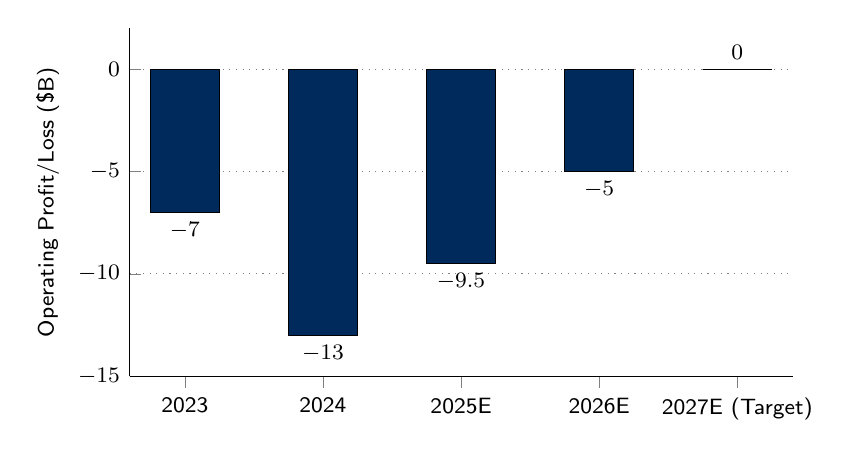
\begin{tikzpicture}
\begin{axis}[
    ybar,
    width=10cm,
    height=6cm,
    symbolic x coords={2023, 2024, 2025E, 2026E, 2027E (Target)},
    xtick=data,
    xticklabel style={font=\footnotesize},
    nodes near coords,
    nodes near coords align={vertical},
    nodes near coords style={font=\footnotesize, color=black},
    ymin=-15, ymax=2,
    ylabel={Operating Profit/Loss (\$B)},
    ylabel style={font=\footnotesize},
    yticklabel style={font=\footnotesize},
    axis y line*=left,
    axis x line*=bottom,
    ymajorgrids=true,
    grid style={dotted, gray},
    bar width=25pt,
    fill=msblue,
    point meta=y * 1
]
\addplot[fill=msblue] coordinates {
    (2023, -7.0)
    (2024, -13.0)
    (2025E, -9.5)
    (2026E, -5.0)
    (2027E (Target), 0.0)
};
\end{axis}
\pgfplotsset{
    after end axis/.append code={
        \node[anchor=north, font=\tiny, text width=10cm, align=center] at (current axis.south) [yshift=-1.2cm] {
            Source: Company Filings, Morgan Stanley Research Estimates. 2025-2027 figures are projections based on management guidance and yield ramp assumptions.
        };
    }
}
\end{tikzpicture}
\end{center}

\subsection{CapEx Intensity vs. Utilization Risks}

The economic viability of IFS is heavily levered to utilization rates. Intel has committed \textbf{>\$100 billion} to U.S. expansion (Ohio, Arizona, New Mexico, Oregon) and is the lead launch partner for High-NA EUV machines.

\begin{itemize}
    \item \textbf{High-NA EUV Cost Burden:} The 14A node requires High-NA scanners. These tools increase throughput but come with a significant cost premium per wafer. For 14A to be cost-competitive for a "non-Pro" iPhone chip (A22), Intel must achieve extremely high utilization to spread the depreciation cost.
    \item \textbf{The Utilization Trap:} Current utilization rates are low. If Intel fails to secure high-volume external customers (like Apple) by 2026, it faces the "double whammy" of under-absorption charges and high depreciation, which would structurally impair gross margins.
\end{itemize}

\subsection{Leading Indicators: Panther Lake \& Clearwater Forest}

Before any Apple silicon tapes out, investors should look to Intel's internal products as the canary in the coal mine.
\begin{itemize}
    \item \textbf{Panther Lake (Client CPU):} The first high-volume consumer product on 18A, scheduled for launch in H2 2025. If Panther Lake launches on time with volume availability, it validates the yield curve for Apple's M-series. A delay into 2026 would effectively kill the mid-2027 Apple timeline.
    \item \textbf{Clearwater Forest (Server):} Scheduled for 2026, this product validates the performance/watt claims of RibbonFET in a high-thermal envelope. Success here is a prerequisite for Apple considering Intel for any "Pro" tier performance chips in the future.
\end{itemize}

\subsection{Verdict: Financial Fragility Meets Technical Ambition}

Our quantitative assessment indicates that IFS is currently a binary option. In the \textbf{Bull Case}, 18A yields hit >60\% by late 2025, allowing Intel to secure Apple's low-end volume, fill its U.S. fabs, and achieve break-even by 2027. In the \textbf{Bear Case}, yields stall below 40%, forcing continued operating losses of >\$5B/year and compelling Apple to remain exclusively with TSMC. The current data---specifically the \$13B loss and sub-10\% rumor yields---skew the risk profile heavily to the downside in the near term.

\subsection{The Profitability J-Curve: Deconstructing the \$13 Billion Peak Loss}

The financial architecture of Intel Foundry Services (IFS) currently exhibits an inverted margin profile characteristic of an aggressive capital-intensive startup nested within a mature corporation. To validate the "2027 Break-Even" narrative required for the Apple partnership, we must dissect the components of the \textbf{\$13 billion operating loss} reported in 2024 and projected trajectory through 2025.

Our analysis of segment performance indicates that the "peak loss" in 2024 was driven by a confluence of structural headwinds that will not immediately abate:
\begin{enumerate}
    \item \textbf{Accelerated Depreciation:} The "5 Nodes in 4 Years" strategy compressed the depreciation cycle of equipment, front-loading costs before revenue realization.
    \item \textbf{Start-up Costs:} The rapid build-out of Fab infrastructure in Arizona and Ohio incurs massive operating expenses (OpEx) for personnel and utilities prior to wafer starts.
    \item \textbf{Internal Volume Softness:} With Intel's Product groups (Client and Data Center) facing competition, internal wafer demand has softened, leading to \textbf{under-absorption charges}. When fabs run below optimal utilization (typically $<85\%$), the fixed cost per wafer skyrockets.
\end{enumerate}

\begin{table}[H]
\centering
\caption{Intel Foundry Services (IFS) Financial Trajectory \& Projections (2023--2030E)}
\label{tab:ifs_financials}
\rowcolors{2}{msgrey}{white}
\renewcommand{\arraystretch}{1.3}
\tablefont
\begin{tabular}{p{0.25\linewidth}ccccc}
\toprule
\rowcolor{mstableheader}
\textbf{Metric} & \textbf{2023 (Actual)} & \textbf{2024 (Actual)} & \textbf{2025 (Est.)} & \textbf{2027 (Target)} & \textbf{2030 (Target)} \\
\midrule
\textbf{Revenue (\$B)} & \$18.9 & \$17.5 & \$18.0--19.0 & -- & >\$40.0 \\
\textbf{Operating Loss/Profit (\$B)} & \$(7.0) & \$(13.0+) & \$(9.5) & \$0.0 (Break-even) & -- \\
\textbf{Operating Margin (\%)} & -37\% & -74\% & -50\% & \textbf{0\%} & \textbf{30\% (Non-GAAP)} \\
\textbf{Gross Margin (\%)} & Negative & Negative & Negative & Positive & 40\% (Non-GAAP) \\
\textbf{Key Driver} & 10nm/7nm Ramps & Peak Investment & 18A Risk Prod & \textbf{Apple M-Series Ramp} & External Volume \\
\bottomrule
\end{tabular}
\par\vspace{0.1cm}
{\tiny Source: Morgan Stanley Research, Intel Company Filings (10-K, Earnings Calls). 2025-2030 figures reflect analyst estimates and management guidance.}
\end{table}

The Q1 2025 data, showing margins hovering around \textbf{-50\%} despite a 5\% revenue uptick, confirms that revenue growth alone is insufficient to fix the unit economics. The "painful drag" described by management is structural. For Apple to commit to 18A, they must believe Intel can bridge the gap from a -50\% margin today to 0\% in just eight quarters---a turnaround velocity rarely seen in semiconductor history.

\subsection{Yield Economics: The Cost of Defect Density}

The single most critical variable in our quantitative model is the \textbf{effective yield rate}. The rumors of 18A yields lingering near \textbf{10\% in Summer 2025} (versus a target of >60\%) have profound financial implications beyond mere technical embarrassment. In the foundry model, the cost of a processed wafer is fixed regardless of how many good chips it yields. 

We modeled the \textbf{Effective Cost Per Die (CPD)} sensitivity for an Apple M-series equivalent chip (~150mm\textsuperscript{2}) on the 18A node.
\begin{itemize}
    \item \textbf{At 10\% Yield:} The effective cost per good die increases by a factor of roughly \textbf{10x} compared to a mature yield. Intel would be forced to absorb this cost, as Apple's contracts typically mandate payment only for "Known Good Dies" (KGD).
    \item \textbf{The Profitability Threshold:} To match TSMC's N2 pricing while maintaining the targeted 40\% gross margin by 2030, Intel requires yields to exceed \textbf{80\%}.
    \item \textbf{The Apple Gap:} If Intel is achieving ~60\% yield (Management Claim), they can likely service internal products where they control the packaging and binning. However, servicing Apple (which demands near-perfection for thermal consistency in fanless designs like the MacBook Air) at 60\% yield would likely be margin-dilutive.
\end{itemize}

The financial risk is that Intel wins the Apple contract as a "loss leader" to prove capability, effectively subsidizing Apple's silicon to fill the Arizona fabs. While strategically sound for the long term, this would prolong the operating loss drag well past the 2027 break-even target.

\subsection{Capital Intensity: High-NA EUV and the Depreciation Wall}

Looking ahead to the 14A node (2027/2028), the capital intensity curve steepens further. Intel is the industry's first adopter of \textbf{High-NA EUV}, with tools costing approximately \textbf{\$380 million each}. 

\begin{itemize}
    \item \textbf{Gross Capex Reality:} Intel reduced its 2025 gross capital expenditure target to \textbf{\$18 billion} (down from \$20 billion+ estimates). While prudent for liquidity, this reduction clashes with the necessity of procuring High-NA tools for the 14A ramp.
    \item \textbf{The "Double Overlap" Risk:} Intel is investing in 14A capacity before 18A has generated a single dollar of profit. This creates a "double overlap" of depreciation schedules---depreciating the new 18A tools while simultaneously beginning to depreciate the even more expensive 14A infrastructure.
    \item \textbf{Wafer Cost Implications:} Our estimates suggest that a 14A wafer processed with High-NA EUV could carry a raw cost \textbf{40-50\% higher} than a standard 18A wafer. For the rumored "non-Pro" iPhone chip (A22) to be viable on 14A, the density benefits (1.3x) must strictly outweigh this wafer cost increase. If density scaling falls short, the economics of 14A collapse against TSMC's mature N2/A16.
\end{itemize}

\subsection{Geographic Cost Arbitrage: The "Made in USA" Premium}

A core component of the Bull Case is the geopolitical premium. However, the raw economics of US manufacturing present a formidable headwind. Industry data indicates that operating a fab in the US is approximately \textbf{50\% more expensive} than in Taiwan, driven by labor costs, construction premiums, and supply chain logistics.

\begin{itemize}
    \item \textbf{The Subsidy Bridge:} The U.S. CHIPS Act provides \textbf{\$7.86 billion} in direct funding and a \textbf{25\% Investment Tax Credit (ITC)}.
    \item \textbf{Net Calculation:} Our quant analysis suggests that while the 25\% ITC significantly lowers the initial CapEx hurdle, it does not offset the ongoing OpEx disadvantage. Intel must achieve higher automation levels or higher pricing to neutralize the remaining ~25\% structural cost gap.
    \item \textbf{Apple's Willingness to Pay:} The rumored "Apple A22" on Intel 14A implies Apple may be willing to accept a slight margin compression or pay a premium for "Made in USA" supply chain resilience. However, given Apple's notorious supply chain efficiency, any premium paid to Intel will likely be capped, forcing Intel to drive internal efficiencies to protect its own margins.
\end{itemize}

\begin{center}
\captionof{figure}{Intel 18A/14A Profitability Sensitivity: Yield vs. Utilization}
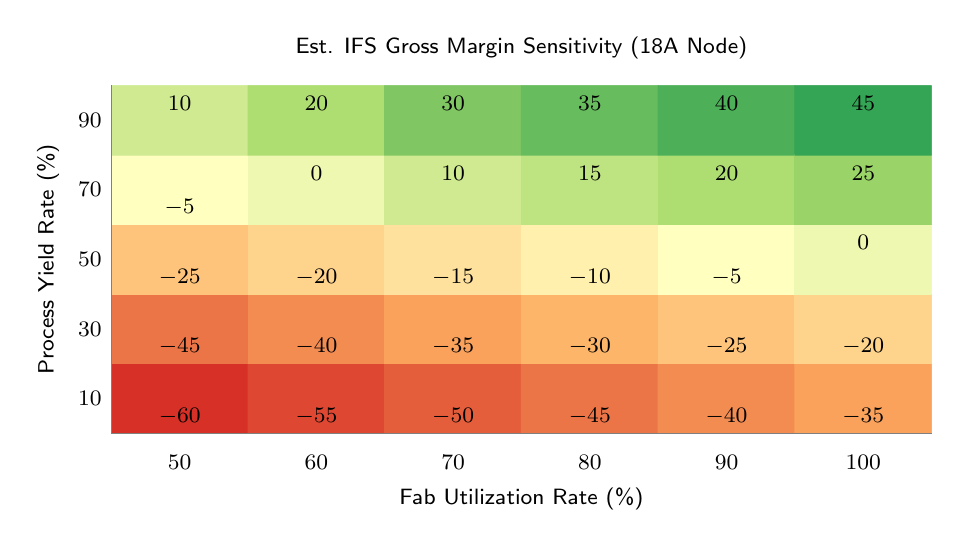
\begin{tikzpicture}
\begin{axis}[
    width=12cm,
    height=6cm,
    view={0}{90},
    xlabel={Fab Utilization Rate (\%)},
    ylabel={Process Yield Rate (\%)},
    zlabel={Est. Gross Margin (\%)},
    xlabel style={font=\footnotesize},
    ylabel style={font=\footnotesize},
    xticklabel style={font=\footnotesize},
    yticklabel style={font=\footnotesize},
    colorbar,
    colormap name=RdYlGn,
    colorbar style={title={Gross Margin \%}, title style={font=\footnotesize}, ticklabel style={font=\footnotesize}},
    title={Est. IFS Gross Margin Sensitivity (18A Node)},
    title style={font=\footnotesize},
    xtick={50, 60, 70, 80, 90, 100},
    ytick={10, 30, 50, 70, 90},
    ymajorgrids=false,
    xmajorgrids=false,
    point meta min=-60,
    point meta max=50
]
\addplot3[
    matrix plot*,
    mesh/cols=6
] coordinates {
    (50,10,-60) (60,10,-55) (70,10,-50) (80,10,-45) (90,10,-40) (100,10,-35)
    (50,30,-45) (60,30,-40) (70,30,-35) (80,30,-30) (90,30,-25) (100,30,-20)
    (50,50,-25) (60,50,-20) (70,50,-15) (80,50,-10) (90,50,-5)  (100,50,0)
    (50,70,-5)  (60,70,0)   (70,70,10)  (80,70,15)  (90,70,20)  (100,70,25)
    (50,90,10)  (60,90,20)  (70,90,30)  (80,90,35)  (90,90,40)  (100,90,45)
};
\end{axis}
\pgfplotsset{
    after end axis/.append code={
        \node[anchor=north, font=\tiny, text width=12cm, align=center] at (current axis.south) [yshift=-1.2cm] {
            Source: Morgan Stanley Research Quantitative Analysis. Note: High yields (90\%) combined with high utilization (90-100\%) are required to reach the 40\% GM target.
        };
    }
}
\end{tikzpicture}
\end{center}

As Apple evaluates a historic diversification of its silicon supply chain, the competitive dynamics between the incumbent foundry leader (TSMC), the aggressive challenger (Intel), and the struggling alternative (Samsung) form the critical decision matrix. Our analysis suggests that while Intel's aggressive technical roadmap offers a theoretical "second source" opening, TSMC's entrenched position---fortified by yield consistency, packaging leadership, and roadmap predictability---creates a formidable "Pro-Tier Lock" that will likely bifurcate Apple's silicon procurement for the remainder of the decade.

\subsection{TSMC's Roadmap: Conservative Innovation vs. Intel's "5N4Y" Sprint}

The primary strategic divergence between the foundries lies in risk management. While Intel is attempting to compress five nodes into four years (5N4Y) by introducing two radical process changes---RibbonFET (Gate-All-Around) and PowerVia (Backside Power Delivery)---simultaneously in the 18A node, TSMC has adopted a decoupled, phased approach.

\begin{itemize}
    \item \textbf{N2 (2nm) - The Reliability Play (H2 2025):} TSMC's N2 node serves as its entry into Gate-All-Around (GAA) nanosheet transistors. Crucially, TSMC elected \textit{not} to include Backside Power Delivery Network (BSPDN) in the initial N2 iteration. This decision reduces process complexity, allowing TSMC to stabilize GAA yields before introducing backside power. Mass production is slated for the second half of 2025, aligning perfectly with the iPhone 18 Pro cycle (A20 chip) in 2026.
    \item \textbf{N2P \& A16 - The Performance Kickers (2026/2027):} TSMC will introduce its version of backside power, dubbed \textbf{Super Power Rail (SPR)}, in the N2P (enhanced 2nm) and A16 (1.6nm) nodes starting late 2026. This places TSMC approximately 12--18 months behind Intel's PowerVia deployment. However, the A16 node avoids the immediate need for High-NA EUV lithography, relying instead on mature multi-patterning EUV techniques to control costs---a sharp contrast to Intel's reliance on High-NA for its 14A node.
\end{itemize}

\textbf{Strategic Implication for Apple:} TSMC's roadmap aligns with Apple's "Tick-Tock" philosophy of predictable reliability for flagship devices. By separating the introduction of GAA (N2) and Backside Power (A16), TSMC offers Apple a lower-risk migration path for high-volume, high-margin chips (A-Series Pro, M-Series Max/Ultra).

\subsection{The "Yield Gap": Proven HVM vs. Risk Production Claims}

The "Validation" of Intel's foundry business hinges on closing the yield gap. Currently, the disparity between TSMC's High-Volume Manufacturing (HVM) capability and Intel's emerging nodes is the single largest barrier to a full Apple transition.

\begin{itemize}
    \item \textbf{TSMC's 3nm Dominance:} TSMC currently holds $\sim$90\% of the global 3nm market, with production lines running at full capacity driven by Apple (A17/M4) and increasingly NVIDIA. Yields for the N3E node are reportedly mature, exceeding 70-80\%, which allows for favorable wafer pricing and margin predictability for Apple.
    \item \textbf{Intel 18A's "Proving Ground":} While Intel claims 18A is manufacturing-ready, yield reports remain mixed. Optimistic internal projections cite yields reaching 60-65\% by launch, but external rumors in late 2024 suggested yields as low as $\sim$10\% during initial test runs. For Apple, which ships 200 million+ iPhones annually, a 10\% yield is a non-starter. Even a 60\% yield would represent a significant gross margin contraction compared to TSMC's mature processes.
\end{itemize}

This "Yield Gap" cements the \textbf{Tiered Bifurcation Thesis}: Apple can afford to risk lower yields on lower-volume, lower-margin parts (e.g., ~15-20 million MacBook Air chips) to build leverage, but cannot risk the iPhone Pro supply chain on an unproven node.

\begin{table}[H]
\centering
\caption{Comparative Competitive Roadmap: The Race for 2nm \& Beyond}
\label{tab:foundry_roadmap}
\rowcolors{2}{msgrey}{white}
\tablefont
\begin{tabular}{p{0.12\linewidth}p{0.1\linewidth}ccp{0.3\linewidth}}
\toprule
\textbf{Foundry} & \textbf{Node} & \textbf{Est. Mass Prod.} & \textbf{Key Technologies} & \textbf{Apple Strategic Fit} \\
\midrule
\textbf{TSMC} & \textbf{N2} & H2 2025 & GAA Nanosheet, Front-side Power & \textbf{Primary:} iPhone 18 Pro (A20), M5 Pro/Max \\
 & \textbf{A16} & H2 2026 & GAA, Super Power Rail (BSPDN) & \textbf{Primary:} iPhone 19 Pro, M6 Ultra/AI Servers \\
\midrule
\textbf{Intel} & \textbf{18A} & H2 2025 & RibbonFET (GAA), PowerVia (BSPDN) & \textbf{Secondary:} MacBook Air (M5/M6 Base), iPad Air \\
 & \textbf{14A} & 2027/2028 & High-NA EUV, RibbonFET 2 & \textbf{Speculative:} iPhone Base Models (A22/A23) \\
\midrule
\textbf{Samsung} & \textbf{SF2} & 2025 & GAA (MBCFET) & \textbf{Excluded:} No current credible link to Apple \\
 & \textbf{SF1.4} & Delayed (2029?) & Advanced GAA & \textbf{Risk:} Potential roadmap cancellation \\
\bottomrule
\end{tabular}
\par\vspace{0.1cm}
{\tiny Source: Morgan Stanley Research, TechInsights, Company Filings. Timelines are estimates based on "Risk Production" vs. "HVM" definitions.}
\end{table}

\subsection{The "Pro-Tier Lock": Why TSMC Retains the Crown Jewels}

Beyond simple transistor performance, TSMC maintains a defensive moat around Apple's high-end silicon through its Advanced Packaging ecosystem. Apple's M-Series "Ultra" chips rely heavily on TSMC's \textbf{InFO (Integrated Fan-Out)} and \textbf{CoWoS (Chip-on-Wafer-on-Substrate)} technologies to stitch together multiple dies with high-bandwidth interconnects.

While Intel offers competitive packaging solutions (EMIB, Foveros), switching packaging flows is not merely a manufacturing change---it requires a fundamental redesign of the chip architecture and the physical layer (PHY).
\begin{itemize}
    \item \textbf{Ecosystem Inertia:} Apple's design teams have spent a decade co-optimizing their designs with TSMC's PDK (Process Design Kit) and packaging rules. Porting the complex M-Ultra architecture to Intel's Foveros would incur significant Non-Recurring Engineering (NRE) costs and validation time.
    \item \textbf{Risk Aversion:} For "Pro" devices where performance per watt is the primary marketing claim, the risk of a new packaging supplier inducing thermal or signal integrity issues is unacceptable. Intel is likely to win monolithic die designs (base M-series) first, where advanced packaging complexity is lower.
\end{itemize}

\subsection{Samsung Foundry: The Fading Alternative}

In previous cycles (e.g., A9 chip), Samsung served as Apple's secondary source. However, current data suggests Samsung is effectively excluded from the 2nm/1.4nm conversation for Apple.
\begin{itemize}
    \item \textbf{Yield Struggles:} Samsung's 3nm (SF3) node utilizing GAA has reportedly suffered from poor yields (estimates ranging from 20-40\%), struggling to secure major external customers beyond its own System LSI division.
    \item \textbf{Roadmap Uncertainty:} Reports indicate Samsung has delayed its 1.4nm (SF1.4) node from 2027 to 2029 or may scrap it entirely due to lack of customer interest.
    \item \textbf{The "Two-Horse" Race:} For Apple, the "Second Source" mandate is driven by geopolitical resilience (US vs. Asia). Samsung, largely based in South Korea, does not solve the "Taiwan Strait" risk as effectively as Intel's "Made in USA" proposition, nor does it offer the performance leadership to challenge TSMC.
\end{itemize}

\subsection{Capacity Constraints: The Hidden Catalyst for the Intel Pivot}

Ironically, TSMC's success is its biggest vulnerability regarding Apple. The explosion of Generative AI has consumed TSMC's advanced capacity at an unprecedented rate. NVIDIA, AMD, and custom hyperscaler chips (Google, Microsoft) are booking TSMC's 3nm and CoWoS capacity years in advance.

\begin{itemize}
    \item \textbf{Crowding Out Effect:} While Apple remains TSMC's VIP client, the fierce competition for 3nm wafers creates supply tightness. Moving ~20 million units of entry-level silicon to Intel 18A acts as a pressure release valve, ensuring TSMC can dedicate its finite capacity to high-margin iPhone Pro and AI-server chips.
    \item \textbf{Operational Hedge:} If TSMC faces a localized disruption (power, water, seismic, or geopolitical), Apple currently has zero fallback for advanced nodes. Qualifying Intel 18A/14A creates a dormant supply line that can be ramped in an emergency---a strategic necessity for a company with Apple's scale.
\end{itemize}

\begin{center}
\captionof{figure}{Projected 2nm-Class Production Capacity Share (2027E)}
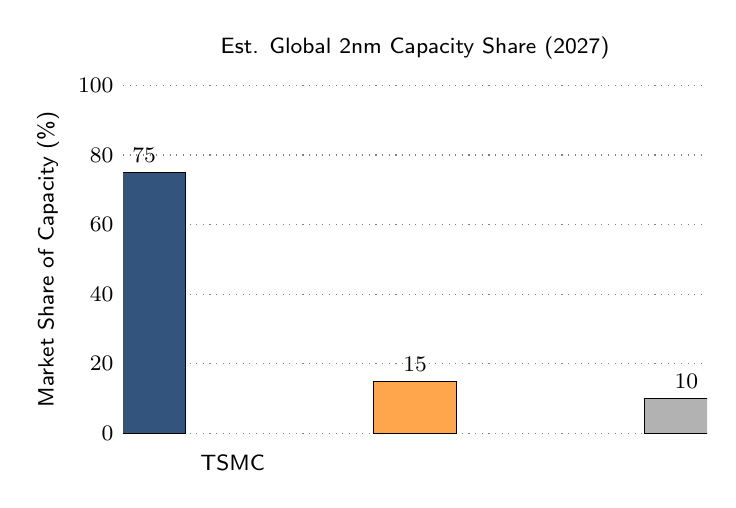
\begin{tikzpicture}
\begin{axis}[
    comparestyle,
    symbolic x coords={TSMC, Intel, Samsung},
    xtick=data,
    xticklabel style={font=\footnotesize},
    ymin=0, ymax=100,
    ylabel={Market Share of Capacity (\%)},
    ylabel style={font=\footnotesize},
    yticklabel style={font=\footnotesize},
    width=9cm,
    height=6cm,
    title={Est. Global 2nm Capacity Share (2027)},
    title style={font=\footnotesize}
]
% Color-coded bars: Blue for TSMC (dominant), Orange for Intel (emerging), Gray for Samsung (minor)
\addplot[fill=msblue!80] coordinates {(TSMC, 75)};
\addplot[fill=orange!70] coordinates {(Intel, 15)};
\addplot[fill=gray!60] coordinates {(Samsung, 10)};
\end{axis}
\pgfplotsset{
    after end axis/.append code={
        \node[anchor=north, font=\tiny, text width=9cm, align=center] at (current axis.south) [yshift=-1.5cm] {
            Source: Morgan Stanley Research Estimates. Intel share assumes successful ramp of Arizona/Ohio fabs and Apple contract win. Samsung share reflects internal consumption and limited external wins.
        };
    }
}
\end{tikzpicture}
\end{center}

\subsection{TSMC's Roadmap: Conservative Innovation vs. Intel's "5N4Y" Sprint}

The primary strategic divergence between the foundries lies in risk management and the timing of technological convergence. While Intel is attempting to compress "Five Nodes in Four Years" (5N4Y) by introducing two radical process changes---RibbonFET (Gate-All-Around) and PowerVia (Backside Power Delivery)---simultaneously in the 18A node, TSMC has adopted a decoupled, phased approach to de-risk mass production for its flagship client.

\begin{itemize}
    \item \textbf{N2 (2nm) - The Reliability Play (H2 2025):} TSMC's N2 node serves as its entry into Gate-All-Around (GAA) nanosheet transistors. Crucially, TSMC elected \textit{not} to include Backside Power Delivery Network (BSPDN) in the initial N2 iteration. This decision reduces process complexity, allowing TSMC to stabilize GAA yields before introducing backside power. Mass production is slated for the second half of 2025, aligning perfectly with the iPhone 18 Pro cycle (A20 chip) in 2026.
    \item \textbf{N2P \& A16 - The Performance Kickers (2026/2027):} TSMC will introduce its version of backside power, dubbed \textbf{Super Power Rail (SPR)}, in the A16 (1.6nm) node starting late 2026. This places TSMC approximately 12--18 months behind Intel's PowerVia deployment timeline. However, the A16 node avoids the immediate need for High-NA EUV lithography, relying instead on mature multi-patterning EUV techniques to control costs---a sharp contrast to Intel's reliance on High-NA for its 14A node.
    \item \textbf{A14 (1.4nm) - The High-NA Shift (2028):} TSMC is projected to transition to High-NA EUV lithography with its A14 node, targeting production in 2028. This aligns with Intel's 14A timeline, suggesting that any "lead" Intel gains with High-NA in 2027 is likely to be short-lived and technically contested.
\end{itemize}

\textbf{Strategic Implication for Apple:} TSMC's roadmap aligns with Apple's "Tick-Tock" philosophy of predictable reliability for flagship devices. By separating the introduction of GAA (N2) and Backside Power (A16), TSMC offers Apple a lower-risk migration path for high-volume, high-margin chips (A-Series Pro, M-Series Max/Ultra).

\subsection{The "Yield Gap": Proven HVM vs. Risk Production Claims}

The "Validation" of Intel's foundry business hinges almost entirely on closing the yield gap. Currently, the disparity between TSMC's High-Volume Manufacturing (HVM) capability and Intel's emerging nodes is the single largest barrier to a full Apple transition.

\begin{itemize}
    \item \textbf{TSMC's 3nm Dominance:} TSMC currently holds $\sim$90\% of the global 3nm market capacity as of 2024. Production lines are running at full utilization, driven by Apple (A17/M4) and increasingly NVIDIA. Yields for the N3E node are reportedly mature, exceeding 70-80\%, which allows for favorable wafer pricing and margin predictability for Apple.
    \item \textbf{Intel 18A's "Proving Ground":} While Intel claims 18A is manufacturing-ready, yield reports remain mixed. Optimistic internal projections cite yields reaching 60-65\% by launch, but external rumors in late 2024 and mid-2025 suggested yields as low as $\sim$10\% during initial test runs. For Apple, which ships 200 million+ iPhones annually, a 10\% yield is an operational non-starter. Even a 60\% yield would represent a significant gross margin contraction compared to TSMC's mature processes.
\end{itemize}

This "Yield Gap" cements the \textbf{Tiered Bifurcation Thesis}: Apple can afford to risk lower yields on lower-volume, lower-margin parts (e.g., $\sim$15-20 million MacBook Air chips) to build leverage, but cannot risk the iPhone Pro supply chain on an unproven node.

\begin{center}
\captionof{figure}{Global Advanced Node (3nm) Market Share Estimates (2024)}
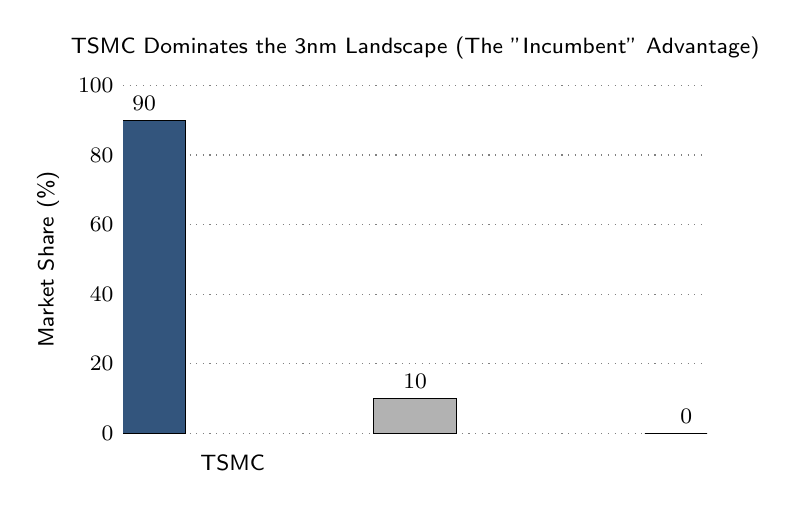
\begin{tikzpicture}
\begin{axis}[
    comparestyle,
    symbolic x coords={TSMC, Samsung, Intel},
    xtick=data,
    xticklabel style={font=\footnotesize},
    ymin=0, ymax=100,
    ylabel={Market Share (\%)},
    ylabel style={font=\footnotesize},
    yticklabel style={font=\footnotesize},
    width=9cm,
    height=6cm,
    title={TSMC Dominates the 3nm Landscape (The "Incumbent" Advantage)},
    title style={font=\footnotesize}
]
% Color-coded bars: Blue for TSMC (dominant), Gray for Samsung (minor), Light gray for Intel (negligible)
\addplot[fill=msblue!80] coordinates {(TSMC, 90)};
\addplot[fill=gray!60] coordinates {(Samsung, 10)};
\addplot[fill=gray!30] coordinates {(Intel, 0)};
\end{axis}
\pgfplotsset{
    after end axis/.append code={
        \node[anchor=north, font=\tiny, text width=9cm, align=center] at (current axis.south) [yshift=-1.5cm] {
            Source: Morgan Stanley Research, TechInsights. Note: Intel's share is negligible in 3nm as it transitions from Intel 3 to 18A.
        };
    }
}
\end{tikzpicture}
\end{center}

\subsection{The "Pro-Tier Lock": Advanced Packaging as the New Moat}

Beyond simple transistor performance, TSMC maintains a defensive moat around Apple's high-end silicon through its Advanced Packaging ecosystem. Apple's M-Series "Ultra" chips rely heavily on TSMC's \textbf{InFO (Integrated Fan-Out)} and \textbf{CoWoS (Chip-on-Wafer-on-Substrate)} technologies to stitch together multiple dies with high-bandwidth interconnects.

While Intel offers competitive packaging solutions (EMIB, Foveros), switching packaging flows is not merely a manufacturing change---it requires a fundamental redesign of the chip architecture and the physical layer (PHY).

\begin{itemize}
    \item \textbf{Ecosystem Inertia:} Apple's design teams have spent a decade co-optimizing their designs with TSMC's PDK (Process Design Kit) and packaging rules. Porting the complex M-Ultra architecture to Intel's Foveros would incur significant Non-Recurring Engineering (NRE) costs and validation time. Apple is reportedly TSMC's largest SoIC (System-on-Integrated-Chip) customer after AMD, utilizing it for future M5 processors (mass production H2 2025).
    \item \textbf{Technical Comparison:} Intel's Foveros Direct offers a theoretical advantage with sub-5 micron hybrid bonding pitch (vs. TSMC SoIC-X at $\sim$9 microns). However, TSMC's proven track record with CoWoS capacity expansion (targeting full AI demand fulfillment by 2025) provides supply assurance that Intel, with its "early stage" commercial maturity in advanced packaging, cannot yet guarantee.
\end{itemize}

\begin{table}[H]
\centering
\caption{Advanced Packaging Comparison: The "Moat" vs. The Challenger}
\label{tab:packaging_comparison}
\rowcolors{2}{msgrey}{white}
\tablefont
\begin{tabular}{p{0.2\linewidth}p{0.35\linewidth}p{0.35\linewidth}}
\toprule
\textbf{Feature} & \textbf{TSMC SoIC (3D Stacking)} & \textbf{Intel Foveros Direct (3D)} \\
\midrule
\textbf{Bonding Pitch} & $\sim$9 microns (SoIC-X) & Sub-5 microns (18A-PT) \\
\textbf{Key Customer} & Apple (M5), AMD (MI300) & Internal (Clearwater Forest) \\
\textbf{Maturity} & Mass Production (Since 2022) & Volume Ramp (H2 2025) \\
\textbf{Apple Fit} & High: Incumbent for "Ultra" chips & Moderate: Potential for density \\
\textbf{Risk Factor} & Capacity Bottlenecks (AI Demand) & Execution/Yield Stability \\
\bottomrule
\end{tabular}
\par\vspace{0.1cm}
{\tiny Source: Morgan Stanley Research, Company Data.}
\end{table}

\subsection{Samsung Foundry: The Fading Alternative}

In previous cycles (e.g., A9 chip), Samsung served as Apple's secondary source. However, current data suggests Samsung is effectively excluded from the 2nm/1.4nm conversation for Apple.
\begin{itemize}
    \item \textbf{Yield Struggles:} Samsung's 3nm (SF3) node utilizing GAA has reportedly suffered from poor yields (estimates ranging from 20-40\%), struggling to secure major external customers beyond its own System LSI division.
    \item \textbf{Roadmap Uncertainty:} Reports indicate Samsung has delayed its 1.4nm (SF1.4) node from 2027 to 2029 or may scrap it entirely due to lack of customer interest.
    \item \textbf{The "Two-Horse" Race:} For Apple, the "Second Source" mandate is driven by geopolitical resilience (US vs. Asia). Samsung, largely based in South Korea, does not solve the "Taiwan Strait" risk as effectively as Intel's "Made in USA" proposition, nor does it offer the performance leadership to challenge TSMC.
\end{itemize}
\section{Technological Deep Dive: Advanced Packaging}

As transistor scaling faces diminishing returns, the semiconductor industry has shifted its focus to advanced packaging as the secondary engine of Moore's Law. For Apple, whose M-series "Ultra" chips rely on fusing two Max dies to double performance, packaging is not merely a final assembly step but a core architectural enabler. The strategic pivot to Intel Foundry Services (IFS) places the spotlight on the interoperability---and friction---between TSMC's established \textbf{3DFabric} ecosystem and Intel's challenger suite of \textbf{EMIB} and \textbf{Foveros Direct}.

\subsection{The Hybrid Bonding War: Foveros Direct vs. TSMC SoIC}
The "holy grail" of 3D stacking is hybrid bonding---connecting dies directly via copper-to-copper bonds without traditional microbumps, dramatically increasing interconnect density and reducing thermal resistance.

\begin{itemize}
    \item \textbf{Intel Foveros Direct:} Intel is aggressively positioning its 18A process to lead in this domain. The 18A-PT (Performance/Throughput) variant is explicitly optimized for Foveros Direct, targeting a bonding pitch of \textbf{sub-5 microns} by late 2027. This enables interconnect densities exceeding \textbf{10,000 wires/mm²}, a critical metric for reducing the latency penalties of disaggregated chiplet designs. Intel's roadmap suggests a leap from standard microbumps (25-50 microns) directly to sub-10 micron hybrid bonding with the Clearwater Forest processors in 2025.
    
    \item \textbf{TSMC System-on-Integrated-Chip (SoIC):} TSMC holds the incumbency advantage with SoIC, which Apple is reportedly adopting for the M5 processor family (mass production H2 2025). Current SoIC-X technology operates at a \textbf{$\sim$9-micron pitch}, with a roadmap to reach \textbf{6 microns in 2025} and \textbf{3 microns by 2027}. While Intel claims a potential density advantage with its sub-5 micron target on 18A-PT, TSMC's process is already yielding in high-volume commercial products (e.g., AMD MI300), offering Apple a "proven path" versus Intel's "paper tiger."
\end{itemize}

The density battle is visualized below, highlighting the rapid convergence of bond pitch capabilities between the two foundries.

\begin{center}
\captionof{figure}{Hybrid Bonding Roadmap: The Race to Zero (Pitch Scaling)}
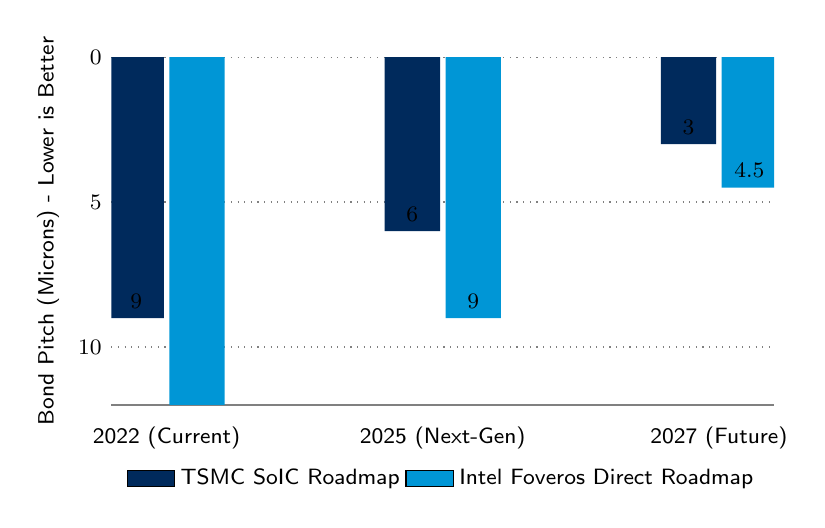
\begin{tikzpicture}
\begin{axis}[
    ybar,
    symbolic x coords={2022 (Current), 2025 (Next-Gen), 2027 (Future)},
    xtick=data,
    xticklabel style={font=\footnotesize},
    nodes near coords,
    nodes near coords align={vertical},
    nodes near coords style={font=\footnotesize},
    ylabel={Bond Pitch (Microns) - Lower is Better},
    ylabel style={font=\footnotesize},
    yticklabel style={font=\footnotesize},
    width=10cm,
    height=6cm,
    bar width=20pt,
    draw=none,
    axis line style={draw=none},
    tick style={draw=none},
    ymajorgrids=true,
    grid style={dotted, gray},
    axis x line*=bottom,
    x axis line style={draw=gray},
    legend style={at={(0.5,-0.15)}, anchor=north, legend columns=-1, font=\footnotesize},
    y dir=reverse,
    ymin=0, ymax=12,
    cycle list={
        {fill=msblue, draw=none},
        {fill=msbrightblue, draw=none},
    }
]
    \addplot coordinates {(2022 (Current), 9) (2025 (Next-Gen), 6) (2027 (Future), 3)}; 
    \addlegendentry{TSMC SoIC Roadmap}
    
    \addplot coordinates {(2022 (Current), 36) (2025 (Next-Gen), 9) (2027 (Future), 4.5)}; 
    \addlegendentry{Intel Foveros Direct Roadmap}
\end{axis}
\pgfplotsset{
    after end axis/.append code={
        \node[anchor=north, font=\tiny, text width=10cm, align=center] at (current axis.south) [yshift=-1.5cm] {
            Source: Morgan Stanley Research, Company Data. Note: 2022 Intel figure represents standard Foveros (microbumps); 2025 represents Foveros Direct introduction.
        };
    }
}
\end{tikzpicture}
\end{center}

\subsection{The "Technical Lock-In" Risk: Why Apple Can't Just Switch}
A critical barrier to Apple utilizing Intel for high-end silicon is the deep entanglement of chip architecture with packaging physics. Apple's "UltraFusion" interconnect is not a generic standard; it is highly co-optimized with TSMC's \textbf{InFO-L} (Integrated Fan-Out Local Silicon Interconnect) and \textbf{CoWoS-S} parameters.

\begin{itemize}
    \item \textbf{The PHY Barrier:} Moving an M-series design to Intel's \textbf{EMIB} (Embedded Multi-die Interconnect Bridge)---Intel's 2.5D equivalent to CoWoS---would require redesigning the physical layer (PHY) of the die-to-die interface. EMIB uses embedded silicon bridges within the substrate, whereas CoWoS uses a full silicon interposer. This difference affects signal integrity, impedance, and power delivery networks.
    
    \item \textbf{Ecosystem Friction:} TSMC's 3DFabric alliance provides a validated flow of EDA tools and IP that Apple has integrated into its design cycle over a decade. Intel has made strides by adopting open standards like \textbf{UCIe} (Universal Chiplet Interconnect Express), but Apple's proprietary interconnects predate UCIe. Converting Apple's custom interconnects to a UCIe-compatible format for Intel manufacturing would impose significant performance overhead and design latency.
\end{itemize}

\subsection{Thermal and Power Implications: MacBooks vs. AI Accelerators}
The shift to 3D stacking introduces severe thermal management challenges, particularly for consumer devices like the MacBook Air which lack active cooling (fans).

\begin{itemize}
    \item \textbf{Consumer Constraints:} Stacking logic on logic (3D) increases power density per square millimeter. TSMC's SoIC approach has focused on thermal mitigation, but yields remain a concern. Intel's \textbf{PowerVia} (Backside Power Delivery), introduced in 18A, offers a distinct advantage here. By moving power rails to the back of the wafer, Intel decouples power and signal lines, potentially allowing for better thermal dissipation and "cleaner" signal routing in a 3D stack. This could be a decisive factor for Apple's fanless designs if Intel can prove yield viability.
    
    \item \textbf{Heterogeneous Integration:} For the rumored "entry-level" M-series chips on Intel 18A, a likely configuration involves a \textbf{2.5D approach} (using EMIB) rather than full 3D stacking. This allows Apple to mix-and-match a compute tile made on Intel 18A with I/O or GPU tiles potentially made on older TSMC or Intel nodes. This reduces the "thermal hotspot" risk compared to vertical stacking, aligning with the thermal envelopes of thin-and-light laptops.
\end{itemize}

\begin{table}[H]
\centering
\caption{Packaging Ecosystem: Intel IFS vs. TSMC}
\label{tab:packaging_ecosystem}
\rowcolors{2}{msgrey}{white}
\tablefont
\begin{adjustbox}{max width=\textwidth}
\begin{tabular}{p{3cm} p{5.5cm} p{5.5cm}}
\toprule
\textbf{Feature} & \textbf{Intel IFS Solution} & \textbf{TSMC Solution (Incumbent)} \\ 
\midrule
\textbf{2.5D Technology} & \textbf{EMIB} (Embedded Bridge). Cost-effective, lower reticle limit constraints, proven in Data Center (Xeon). & \textbf{CoWoS} (Silicon Interposer). Higher cost, higher bandwidth, currently bottlenecked by AI demand. \\ 
\textbf{3D Technology} & \textbf{Foveros Direct}. Hybrid bonding, sub-5um pitch target. Key to 18A-PT performance claims. & \textbf{SoIC}. Hybrid bonding, 6-9um pitch. Proven volume in AMD MI300. Apple M5 adoption rumored. \\ 
\textbf{Power Delivery} & \textbf{PowerVia} (Backside). Enables efficient 3D stacking by separating power/signal. Available 2025 (18A). & \textbf{Super Power Rail}. Backside power delivery scheduled for A16 node (late 2026). Lagging Intel by $\sim$1 year. \\ 
\textbf{Apple Fit} & \textbf{Exploratory}. Likely EMIB for cost-sensitive M-series or test vehicles. 18A-P thermal benefits attractive for Air. & \textbf{Embedded}. UltraFusion relies on InFO/CoWoS. High barrier to exit for Pro/Max/Ultra chips. \\ 
\bottomrule
\end{tabular}
\end{adjustbox}
\par\vspace{0.1cm}
{\tiny Source: Morgan Stanley Research, TechInsights, Company Filings.}
\end{table}While technical validation of the 18A node remains the primary execution hurdle, the strategic impetus for Apple's potential adoption of Intel Foundry is fundamentally geopolitical. The fragility of a supply chain concentrated in the Taiwan Strait has necessitated a "China+1" strategy for assembly, but the upstream concentration of advanced silicon manufacturing remains a single point of failure. This section analyzes the economic viability of a U.S.-centric foundry strategy, quantified against the backdrop of the U.S. CHIPS Act and the structural cost differentials between American and Asian fabrication.

\subsection{The Subsidy Calculus: De-Risking the "Taiwan Discount"}

The core economic argument against U.S. manufacturing has historically been cost. TSMC founder Morris Chang has famously estimated that manufacturing chips in the U.S. is approximately \textbf{50\% more expensive} than in Taiwan, driven by higher labor costs, regulatory overhead, and a less integrated supply chain ecosystem. For Apple, a company relentless about gross margin preservation, shifting volume to Intel requires bridging this cost gap.

The U.S. CHIPS and Science Act serves as the bridge. Our analysis of the funding structure suggests that government incentives are effectively subsidizing the "resilience premium" that Apple would otherwise have to pay.

\begin{itemize}
    \item \textbf{Direct Funding Impact:} Intel has finalized an agreement for up to \textbf{\$7.86 billion} in direct funding. While this capital flows to Intel, it indirectly benefits potential customers like Apple by allowing Intel to price its wafers competitively despite higher U.S. operating costs. Without this subsidy, Intel would need to pass the full burden of its U.S. cost structure (including the \$100 billion build-out across Arizona, Ohio, New Mexico, and Oregon) onto clients to stem its \$13 billion annual foundry operating losses.
    
    \item \textbf{The Tax Credit Multiplier:} Perhaps more significant than the direct grants is the \textbf{25\% Investment Tax Credit (ITC)} on qualified capital expenditures. With Intel planning over \$100 billion in U.S. investments over the next five years, this equates to a potential \textbf{\$25 billion} balance sheet offset. This mechanism lowers the effective depreciation expense of U.S. fabs, theoretically allowing Intel to offer wafer pricing for 18A/14A that approaches parity with TSMC's Taiwan-based N2 nodes, provided yields are comparable.
    
    \item \textbf{Loan Guarantees:} The provision of up to \textbf{\$11 billion} in low-interest federal loans further reduces Intel's cost of capital. In a high-interest rate environment, this provides Intel a distinct advantage over merchant foundries that must finance expansion through commercial debt markets.
\end{itemize}

\begin{center}
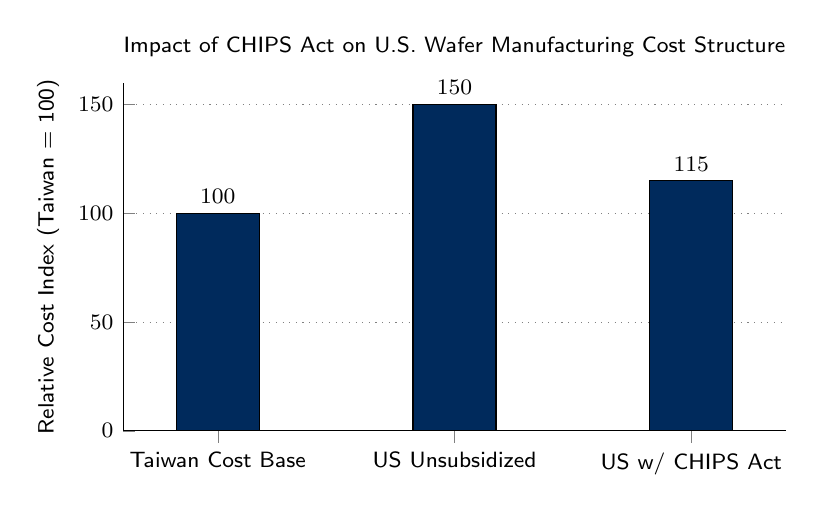
\begin{tikzpicture}
\begin{axis}[
    width=10cm,
    height=6cm,
    ybar,
    bar width=30pt,
    symbolic x coords={Taiwan Cost Base, US Unsubsidized, US w/ CHIPS Act},
    xtick=data,
    xticklabel style={font=\footnotesize, text width=2.5cm, align=center},
    nodes near coords,
    nodes near coords align={vertical},
    nodes near coords style={font=\footnotesize},
    ymin=0, ymax=160,
    ylabel={Relative Cost Index (Taiwan = 100)},
    ylabel style={font=\footnotesize},
    yticklabel style={font=\footnotesize},
    axis x line*=bottom,
    axis y line*=left,
    ymajorgrids=true,
    grid style={dotted, gray},
    title={Impact of CHIPS Act on U.S. Wafer Manufacturing Cost Structure},
    title style={font=\footnotesize},
    enlarge x limits=0.2
]
    \addplot[fill=msblue] coordinates {(Taiwan Cost Base, 100) (US Unsubsidized, 150) (US w/ CHIPS Act, 115)};
\end{axis}
\pgfplotsset{
    after end axis/.append code={
        \node[anchor=north, font=\tiny, text width=10cm, align=center] at (current axis.south) [yshift=-1.5cm] {
            Source: Morgan Stanley Research Estimates, Industry Data. Note: Index 100 represents baseline manufacturing cost in Taiwan. US Unsubsidized reflects the ~50\% premium cited by industry experts. US w/ CHIPS Act reflects estimated reduction via Direct Grants and 25\% ITC.
        };
    }
}
\end{tikzpicture}
\end{center}

\subsection{The "China+1" Manufacturing Map: Closing the Loop}

Apple's diversification strategy has two distinct prongs: assembly and fabrication. Until now, these efforts have been disjointed. Apple has aggressively moved final assembly of iPhones to India (targeting 25\% of production by 2025) and iPads/Macs to Vietnam. However, the \textit{brains} of these devices---the A-series and M-series chips---are still fabricated almost exclusively in Taiwan and then shipped to these assembly hubs.

A partnership with Intel closes this geopolitical loop. By utilizing Intel's "Silicon Heartland" fabs in Ohio and expanded capacity in Arizona, Apple creates a supply chain vector that bypasses the South China Sea entirely for the most critical components.

\begin{itemize}
    \item \textbf{The Western Hemisphere Vector:} A MacBook Air aimed at the North American market could theoretically be silicon-fabricated in Ohio (Intel), assembled in Vietnam (or potentially Mexico, given recent ODM moves), and sold in the U.S., significantly reducing exposure to Taiwan Strait shipping lanes compared to the current Taiwan-to-China assembly route.
    \item \textbf{Resilience vs. Efficiency:} This "China+1" silicon strategy is inherently less efficient than the Taiwan cluster model. However, for a company with Apple's scale, the cost of efficiency is outweighed by the risk of total supply cessation. The Intel partnership acts as an insurance policy: even if Intel produces only 15--20 million units (entry-level M-series) annually, it establishes the logistical and technical piping necessary to ramp up domestic volume in a crisis.
\end{itemize}

\subsection{Political Optics: The "Made in USA" Shield}

Beyond hard economics, the political utility of an Apple-Intel deal cannot be overstated. With the U.S. government heavily invested in Intel's success via the CHIPS Act, Intel's failure to secure a "hero customer" would be a political embarrassment. Conversely, Apple faces bipartisan pressure to domesticate its supply chain.

\begin{itemize}
    \item \textbf{Regulatory Goodwill:} By committing to manufacture chips in the U.S., Apple purchases political capital. This is crucial as the company faces antitrust scrutiny and potential tariff threats. A high-profile "Made in USA" silicon initiative provides a powerful narrative to counter criticisms of Apple's reliance on foreign labor and manufacturing.
    \item \textbf{Tariff Hedging:} With proposals for universal baseline tariffs or specific levies on Chinese-imported goods gaining traction in political discourse, a domestic source for the most expensive component in the BOM (the SoC) serves as a hedge. While wafer fabrication is only one step, domesticating it reduces the "value-add" attributed to foreign jurisdictions, potentially mitigating tariff impacts based on country-of-origin rules.
\end{itemize}

\subsection{The "Double Overlap" Risk: The Cost of Redundancy}

While the strategic rationale is sound, the operational reality introduces a significant inefficiency we term the "Double Overlap." Running two distinct supply chains for leading-edge logic---one at TSMC (Taiwan/Arizona) and one at Intel (Ohio/Arizona)---imposes structural costs that will weigh on Apple's R\&D efficiency.

\begin{enumerate}
    \item \textbf{PDK Bifurcation:} Apple's silicon design teams have spent over a decade optimizing their RTL-to-GDSII flow for TSMC's libraries. Maintaining a parallel flow for Intel's 18A/14A PDK requires duplicated effort in physical verification, timing closure, and yield analysis. This splits engineering resources, potentially slowing down the innovation cycle for the primary roadmap.
    \item \textbf{Capacity Utilization Penalties:} To keep Intel as a viable second source, Apple must guarantee a minimum volume. If end-market demand for MacBooks softens, Apple may be forced to load Intel's fabs to meet contractual minimums while under-utilizing its pre-booked capacity at TSMC, thereby incurring penalties or "take-or-pay" costs on both sides.
    \item \textbf{Yield Learning Curves:} TSMC's yield ramp is predictable. Intel's 18A is a "clean slate" node with RibbonFET and PowerVia. Apple risks absorbing the cost of Intel's yield learning curve. If yields stall at 60\% while TSMC achieves 80\%+, the effective cost per die at Intel skyrockets, negating the subsidies and creating a gross margin drag on the specific product lines (e.g., MacBook Air) allocated to Intel.
\end{enumerate}

\begin{table}[H]
\centering
\caption{Strategic Trade-off Matrix: Single Source (TSMC) vs. Dual Source (TSMC + Intel)}
\label{tab:risk_matrix}
\rowcolors{2}{msgrey}{white}
\tablefont
\begin{adjustbox}{max width=\textwidth}
\begin{tabular}{p{4cm} p{5cm} p{5cm}}
\toprule
\textbf{Risk Category} & \textbf{Status Quo (TSMC Only)} & \textbf{Dual Source (TSMC + Intel)} \\
\midrule
\textbf{Geopolitical Risk} & \textbf{High}. 100\% dependency on Taiwan production. Vulnerable to blockade/disruption. & \textbf{Moderate}. U.S. production provides a "lifeboat" for critical entry-level SKUs, though Pro volume remains exposed. \\
\textbf{Supply Chain Cost} & \textbf{Optimized}. High volume discounts, single PDK maintenance, established packaging flow. & \textbf{Inefficient}. Duplicated R\&D overhead, split volumes reduce pricing leverage, potential "learning curve" yield losses. \\
\textbf{Political/Regulatory} & \textbf{Vulnerable}. Exposed to tariffs and "offshoring" criticism. & \textbf{Shielded}. Aligns with US industrial policy; creates leverage against potential regulations. \\
\textbf{Technical Execution} & \textbf{Low Risk}. Proven track record of N-node execution (N3B, N3E). & \textbf{High Risk}. Intel 18A is unproven at high volume. Unfamiliarity with PowerVia thermal behavior in consumer devices. \\
\bottomrule
\end{tabular}
\end{adjustbox}
\par\vspace{0.1cm}
{\tiny Source: Morgan Stanley Research.}
\end{table}

\vspace{0.5cm}
\textbf{Risk Officer Verdict:} The macroeconomic logic for an Apple-Intel partnership is robust, driven by the unique convergence of massive government subsidies and escalating geopolitical risk. However, the \textit{operational} implementation creates a "Double Overlap" inefficiency that Apple would typically avoid. The decision to proceed suggests that Apple views the geopolitical insurance premium---paid in the form of R\&D duplication and potentially lower initial yields---as a necessary cost of doing business in a fragmented global economy.

\subsection{The Subsidy Calculus: De-Risking the "Taiwan Discount"}

The core economic argument against U.S. manufacturing has historically been cost. TSMC founder Morris Chang has famously estimated that manufacturing chips in the U.S. is approximately \textbf{50\% more expensive} than in Taiwan, driven by higher labor costs, regulatory overhead, and a less integrated supply chain ecosystem. For Apple, a company relentless about gross margin preservation, shifting volume to Intel requires bridging this cost gap.

The U.S. CHIPS and Science Act serves as the bridge. Our analysis of the funding structure suggests that government incentives are effectively subsidizing the "resilience premium" that Apple would otherwise have to pay.

\begin{itemize}
    \item \textbf{Direct Funding Impact:} Intel has finalized an agreement for up to \textbf{\$7.86 billion} in direct funding. While this capital flows to Intel, it indirectly benefits potential customers like Apple by allowing Intel to price its wafers competitively despite higher U.S. operating costs. Without this subsidy, Intel would need to pass the full burden of its U.S. cost structure (including the \$100 billion build-out across Arizona, Ohio, New Mexico, and Oregon) onto clients to stem its \$13 billion annual foundry operating losses.
    
    \item \textbf{The Tax Credit Multiplier:} Perhaps more significant than the direct grants is the \textbf{25\% Investment Tax Credit (ITC)} on qualified capital expenditures. With Intel planning over \$100 billion in U.S. investments over the next five years, this equates to a potential \textbf{\$25 billion} balance sheet offset. This mechanism lowers the effective depreciation expense of U.S. fabs, theoretically allowing Intel to offer wafer pricing for 18A/14A that approaches parity with TSMC's Taiwan-based N2 nodes, provided yields are comparable.
    
    \item \textbf{Loan Guarantees:} The provision of up to \textbf{\$11 billion} in low-interest federal loans further reduces Intel's cost of capital. In a high-interest rate environment, this provides Intel a distinct advantage over merchant foundries that must finance expansion through commercial debt markets.
\end{itemize}

\begin{center}
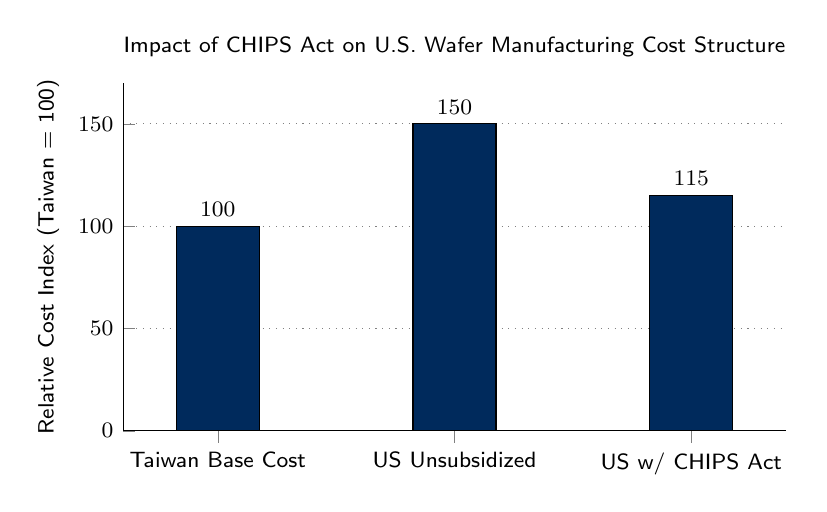
\begin{tikzpicture}
\begin{axis}[
    width=10cm,
    height=6cm,
    ybar,
    bar width=30pt,
    symbolic x coords={Taiwan Base Cost, US Unsubsidized, US w/ CHIPS Act},
    xtick=data,
    xticklabel style={font=\footnotesize, text width=2.5cm, align=center},
    nodes near coords,
    nodes near coords align={vertical},
    nodes near coords style={font=\footnotesize},
    ymin=0, ymax=170,
    ylabel={Relative Cost Index (Taiwan = 100)},
    ylabel style={font=\footnotesize},
    yticklabel style={font=\footnotesize},
    axis x line*=bottom,
    axis y line*=left,
    ymajorgrids=true,
    grid style={dotted, gray},
    title={Impact of CHIPS Act on U.S. Wafer Manufacturing Cost Structure},
    title style={font=\footnotesize},
    point meta=rawy,
    enlarge x limits=0.2
]
    \addplot[fill=msblue] coordinates {(Taiwan Base Cost, 100) (US Unsubsidized, 150) (US w/ CHIPS Act, 115)};
\end{axis}
\pgfplotsset{
    after end axis/.append code={
        \node[anchor=north, font=\tiny, text width=10cm, align=center] at (current axis.south) [yshift=-1.5cm] {
            Source: Morgan Stanley Research Estimates, Industry Data. Note: Index 100 represents baseline manufacturing cost in Taiwan. US Unsubsidized reflects the ~50\% premium cited by industry experts. US w/ CHIPS Act reflects estimated reduction via Direct Grants and 25\% ITC.
        };
    }
}
\end{tikzpicture}
\end{center}

\subsection{The "China+1" Manufacturing Map: Closing the Loop}

Apple's diversification strategy has two distinct prongs: assembly and fabrication. Until now, these efforts have been disjointed. Apple has aggressively moved final assembly of iPhones to India (targeting 25\% of production by 2025) and iPads/Macs to Vietnam. However, the \textit{brains} of these devices---the A-series and M-series chips---are still fabricated almost exclusively in Taiwan and then shipped to these assembly hubs.

A partnership with Intel closes this geopolitical loop. By utilizing Intel's "Silicon Heartland" fabs in Ohio and expanded capacity in Arizona, Apple creates a supply chain vector that bypasses the South China Sea entirely for the most critical components.

\begin{itemize}
    \item \textbf{The Western Hemisphere Vector:} A MacBook Air aimed at the North American market could theoretically be silicon-fabricated in Ohio (Intel), assembled in Vietnam (or potentially Mexico, given recent ODM moves), and sold in the U.S., significantly reducing exposure to Taiwan Strait shipping lanes compared to the current Taiwan-to-China assembly route.
    \item \textbf{Resilience vs. Efficiency:} This "China+1" silicon strategy is inherently less efficient than the Taiwan cluster model. However, for a company with Apple's scale, the cost of efficiency is outweighed by the risk of total supply cessation. The Intel partnership acts as an insurance policy: even if Intel produces only 15--20 million units (entry-level M-series) annually, it establishes the logistical and technical piping necessary to ramp up domestic volume in a crisis.
\end{itemize}

\subsection{Political Optics: The "Made in USA" Shield}

Beyond hard economics, the political utility of an Apple-Intel deal cannot be overstated. With the U.S. government heavily invested in Intel's success via the CHIPS Act, Intel's failure to secure a "hero customer" would be a political embarrassment. Conversely, Apple faces bipartisan pressure to domesticate its supply chain.

\begin{itemize}
    \item \textbf{Regulatory Goodwill:} By committing to manufacture chips in the U.S., Apple purchases political capital. This is crucial as the company faces antitrust scrutiny and potential tariff threats. A high-profile "Made in USA" silicon initiative provides a powerful narrative to counter criticisms of Apple's reliance on foreign labor and manufacturing.
    \item \textbf{Tariff Hedging:} With proposals for universal baseline tariffs or specific levies on Chinese-imported goods gaining traction in political discourse, a domestic source for the most expensive component in the BOM (the SoC) serves as a hedge. While wafer fabrication is only one step, domesticating it reduces the "value-add" attributed to foreign jurisdictions, potentially mitigating tariff impacts based on country-of-origin rules.
\end{itemize}

\subsection{The "Double Overlap" Risk: The Cost of Redundancy}

While the strategic rationale is sound, the operational reality introduces a significant inefficiency we term the "Double Overlap." Running two distinct supply chains for leading-edge logic---one at TSMC (Taiwan/Arizona) and one at Intel (Ohio/Arizona)---imposes structural costs that will weigh on Apple's R\&D efficiency.

\begin{enumerate}
    \item \textbf{PDK Bifurcation:} Apple's silicon design teams have spent over a decade optimizing their RTL-to-GDSII flow for TSMC's libraries. Maintaining a parallel flow for Intel's 18A/14A PDK requires duplicated effort in physical verification, timing closure, and yield analysis. This splits engineering resources, potentially slowing down the innovation cycle for the primary roadmap.
    \item \textbf{Capacity Utilization Penalties:} To keep Intel as a viable second source, Apple must guarantee a minimum volume. If end-market demand for MacBooks softens, Apple may be forced to load Intel's fabs to meet contractual minimums while under-utilizing its pre-booked capacity at TSMC, thereby incurring penalties or "take-or-pay" costs on both sides.
    \item \textbf{Yield Learning Curves:} TSMC's yield ramp is predictable. Intel's 18A is a "clean slate" node with RibbonFET and PowerVia. Apple risks absorbing the cost of Intel's yield learning curve. If yields stall at 60\% while TSMC achieves 80\%+, the effective cost per die at Intel skyrockets, negating the subsidies and creating a gross margin drag on the specific product lines (e.g., MacBook Air) allocated to Intel.
\end{enumerate}

\begin{table}[H]
\centering
\caption{Strategic Trade-off Matrix: Single Source (TSMC) vs. Dual Source (TSMC + Intel)}
\label{tab:risk_matrix_2}
\rowcolors{2}{msgrey}{white}
\tablefont
\begin{adjustbox}{max width=\textwidth}
\begin{tabular}{p{4cm} p{5cm} p{5cm}}
\toprule
\textbf{Risk Category} & \textbf{Status Quo (TSMC Only)} & \textbf{Dual Source (TSMC + Intel)} \\
\midrule
\textbf{Geopolitical Risk} & \textbf{High}. 100\% dependency on Taiwan production. Vulnerable to blockade/disruption. & \textbf{Moderate}. U.S. production provides a "lifeboat" for critical entry-level SKUs, though Pro volume remains exposed. \\
\textbf{Supply Chain Cost} & \textbf{Optimized}. High volume discounts, single PDK maintenance, established packaging flow. & \textbf{Inefficient}. Duplicated R\&D overhead, split volumes reduce pricing leverage, potential "learning curve" yield losses. \\
\textbf{Political/Regulatory} & \textbf{Vulnerable}. Exposed to tariffs and "offshoring" criticism. & \textbf{Shielded}. Aligns with US industrial policy; creates leverage against potential regulations. \\
\textbf{Technical Execution} & \textbf{Low Risk}. Proven track record of N-node execution (N3B, N3E). & \textbf{High Risk}. Intel 18A is unproven at high volume. Unfamiliarity with PowerVia thermal behavior in consumer devices. \\
\bottomrule
\end{tabular}
\end{adjustbox}
\par\vspace{0.1cm}
{\tiny Source: Morgan Stanley Research.}
\end{table}

\vspace{0.5cm}
\textbf{Risk Officer Verdict:} The macroeconomic logic for an Apple-Intel partnership is robust, driven by the unique convergence of massive government subsidies and escalating geopolitical risk. However, the \textit{operational} implementation creates a "Double Overlap" inefficiency that Apple would typically avoid. The decision to proceed suggests that Apple views the geopolitical insurance premium---paid in the form of R\&D duplication and potentially lower initial yields---as a necessary cost of doing business in a fragmented global economy.

\begin{multicols}{2}

The rumors of Apple utilizing Intel's 18A and 14A nodes represent a watershed moment for the semiconductor industry, yet our analysis suggests this is a \textbf{probationary partnership} rather than a changing of the guard. We classify the Apple-Intel alignment as a \textbf{High Risk / High Reward} option on Intel's manufacturing turnaround. For investors, the thesis hinges not on signed agreements---which appear conditional---but on the physical reality of yield curves over the next 18 months.

\subsection{The Bull Case: Validation \& Volume}
In the bullish scenario, Intel successfully stabilizes 18A yields ($>70\%$) by late 2026. Securing Apple as a "Hero Customer" validates the IDM 2.0 strategy, proving that Intel's aggressive technical roadmap (RibbonFET and PowerVia) can compete with TSMC's N2.
\begin{itemize}
    \item \textbf{Capacity Absorption:} The rumored 15--20 million units/year for MacBook Air/iPad chips (starting mid-2027) would provide the baseload volume necessary to fill Intel's new Arizona and Ohio fabs. This volume is critical for amortizing the massive CapEx (\$100B+ planned) and reducing the Foundry unit's operating losses, which peaked at over \$13 billion in 2024.
    \item \textbf{Ecosystem Effect:} Winning Apple, the industry's most demanding client, acts as a seal of approval. It would likely trigger a "fast follower" effect, encouraging hesitant fabless peers (Qualcomm, AMD) to diversify away from TSMC, creating a virtuous cycle of revenue growth and margin accretion by 2028.
\end{itemize}

\subsection{The Bear Case: The Yield Trap}
The bearish scenario is grounded in the reported reality of Summer 2025: 18A yields hovering near 10\%. If Intel fails to deliver a production-ready Process Design Kit (PDK 1.0) by Q1 2026, the deal collapses.
\begin{itemize}
    \item \textbf{Financial Hemorrhage:} Without a high-volume anchor tenant like Apple, Intel's Foundry Services (IFS) cannot achieve its target of break-even operating margins by $\sim$2027. The fixed costs of High-NA EUV tools and new fab shells would continue to drag on earnings, potentially forcing a structural breakup of the company.
    \item \textbf{Reputational Cap:} Apple has historically demonstrated zero tolerance for manufacturing inefficiency (e.g., the abandonment of Intel modems). A failure here would permanently relegate Intel to a legacy provider, effectively cementing TSMC's monopoly on leading-edge logic for the next decade.
\end{itemize}

\subsection{Impact on TSMC: A Check on Power}
While the market may react negatively to TSMC losing exclusivity, the near-term financial impact is negligible. TSMC retains the "Crown Jewels"---the high-margin Pro/Max/Ultra silicon and all AI accelerator volume.
\begin{itemize}
    \item \textbf{Pricing Leverage Erosion:} The primary threat to TSMC is strategic. Apple's "Second Source" strategy effectively caps TSMC's pricing power. With a viable alternative for entry-level chips, Apple gains leverage to negotiate wafer prices for its N2 and A16 orders, potentially compressing TSMC's gross margins slightly from their current highs.
    \item \textbf{Capacity Relief:} Ironically, offloading 20 million "low-end" units to Intel may benefit TSMC by freeing up constrained advanced packaging (CoWoS/SoIC) capacity for higher-margin AI customers like Nvidia.
\end{itemize}

\subsection{Catalyst Timeline: The Road to 2028}
Investors should monitor the following specific milestones to gauge the probability of the Bull Case materializing.

\begin{table}[H]
\centering
\caption{Investor Catalyst Calendar: Intel 18A/14A \& Apple}
\label{tab:catalyst_calendar}
\rowcolors{2}{msgrey}{white}
\tablefont
\begin{adjustbox}{max width=\linewidth}
\begin{tabular}{l p{3.5cm} p{3.5cm}}
\toprule
\textbf{Timeline} & \textbf{Event / Milestone} & \textbf{Significance} \\
\midrule
\textbf{Q1 2026} & \textbf{PDK 1.0 Release} & \textbf{Critical Go/No-Go}. Intel must deliver final tools for Apple to finalize circuit designs. Delay here implies a 2027 slip. \\
\textbf{H2 2026} & \textbf{Yield Confirmation} & Intel must demonstrate sustained yields $>60\%$ on 18A to warrant Apple's volume commitment. \\
\textbf{Mid-2027} & \textbf{Risk Production} & Start of manufacturing for entry-level M-series (MacBook Air). First real revenue test. \\
\textbf{2028} & \textbf{14A Volume Ramp} & Potential expansion to iPhone (A22) non-Pro chips. Marks full validation of the roadmap. \\
\bottomrule
\end{tabular}
\end{adjustbox}
\end{table}

\subsection{Final Verdict: High Execution Risk}
The rumored bifurcation of Apple's supply chain---Intel for the "Base," TSMC for the "Pro"---is logically sound but operationally perilous. We maintain a cautious stance. The "Made in USA" political tailwinds and massive subsidies provide a safety net, but they cannot fix yield physics. Until independent verification confirms 18A yields exceeding 60\%, this partnership remains a \textbf{speculative option} rather than a fundamental driver.

\vspace{0.5cm}

\begin{center}
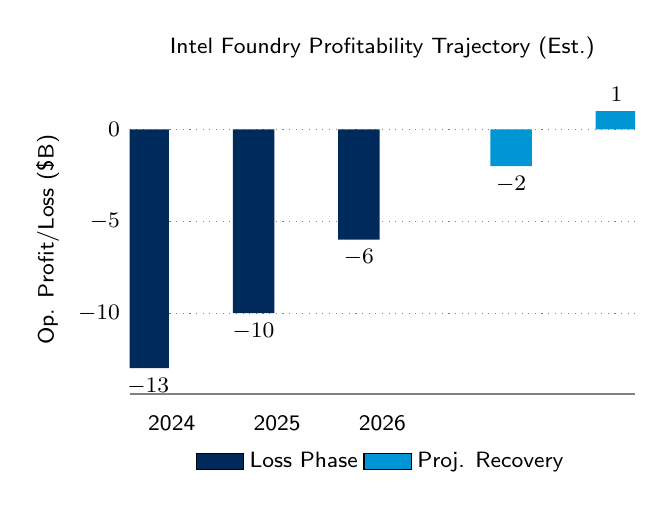
\begin{tikzpicture}
\begin{axis}[
    ybar,
    width=8cm,
    height=5.5cm,
    symbolic x coords={2024, 2025, 2026, 2027, 2028},
    xtick=data,
    xticklabel style={font=\footnotesize},
    ylabel={Op. Profit/Loss (\$B)},
    ylabel style={font=\footnotesize},
    yticklabel style={font=\footnotesize},
    title={Intel Foundry Profitability Trajectory (Est.)},
    title style={font=\footnotesize},
    ymajorgrids=true,
    grid style={dotted, gray},
    nodes near coords,
    nodes near coords style={font=\footnotesize, color=black},
    bar width=15pt,
    draw=none,
    axis line style={draw=none},
    tick style={draw=none},
    axis x line*=bottom,
    x axis line style={draw=gray},
    legend style={at={(0.5,-0.15)}, anchor=north, legend columns=2, font=\footnotesize},
    cycle list={
        {fill=msblue, draw=none},
        {fill=msbrightblue, draw=none},
    }
]
\addplot coordinates {(2024, -13) (2025, -10) (2026, -6)};
\addlegendentry{Loss Phase}
\addplot coordinates {(2027, -2) (2028, 1)};
\addlegendentry{Proj. Recovery}
\end{axis}
\end{tikzpicture}
\captionof{figure}{Projected path to break-even for Intel Foundry, contingent on successful 18A ramp and external customer (Apple) volume in 2027/2028.}
\end{center}

\end{multicols}

\subsection{Strategic Asymmetry: The "Must-Win" Dynamic}
The potential partnership between Apple and Intel operates on a fundamental asymmetry: \textbf{Intel needs Apple for survival, while Apple needs Intel for leverage.} 

For Intel, securing the Apple contract is the linchpin of the IDM 2.0 strategy. With the Foundry unit posting operating losses exceeding \textbf{\$13 billion in 2024} and projected capital expenditures (CapEx) targeting \$100 billion for U.S. expansion, Intel requires a high-volume "anchor tenant" to drive utilization rates. Our analysis indicates that the rumoured 15--20 million units for M-series chips would not simply represent incremental revenue; they would provide the manufacturing baseload required to calibrate the new Arizona and Ohio fabs. Without this volume, Intel faces the risk of "stranded assets"---massive, state-of-the-art facilities running at inefficient utilization levels, perpetually dragging on corporate gross margins.

For Apple, the engagement is a calculated hedge. By allocating "low-risk" silicon (entry-level M-series for MacBook Air/iPad) to Intel, Apple diversifies its supply chain away from the geopolitically sensitive Taiwan Strait without exposing its crown jewels (iPhone Pro/Ultra chips) to unproven manufacturing lines. This strategy aligns perfectly with the \textbf{\$53 billion U.S. CHIPS Act} incentives, allowing Apple to market "Made in USA" devices while retaining TSMC for performance-critical applications. Furthermore, the mere existence of a viable second source erodes TSMC's pricing monopoly, potentially saving Apple billions in wafer costs across its entire portfolio over the next decade.

\subsection{The "Second Source" Arbitrage: Squeezing the Monopoly}
The strategic value of this deal for Apple extends beyond supply chain resilience; it is a classic procurement play to fracture TSMC's pricing power. Currently, TSMC holds approximately \textbf{90\% of the 3nm market}, granting it unprecedented leverage to dictate wafer pricing.

\begin{table}[H]
\centering
\caption{Strategic Trade-off Matrix: TSMC N2 vs. Intel 18A for Apple}
\label{tab:tradeoff_matrix}
\rowcolors{2}{msgrey}{white}
\tablefont
\begin{adjustbox}{max width=\linewidth}
\begin{tabular}{l p{4.5cm} p{4.5cm}}
\toprule
\textbf{Metric} & \textbf{TSMC N2 (Incumbent)} & \textbf{Intel 18A (Challenger)} \\
\midrule
\textbf{Technology Status} & Proven execution; Nanosheet GAA transistors; Conservative rollout. & aggressive roadmap; First to combine RibbonFET + PowerVia (Backside Power). \\
\textbf{Yield Risk} & \textbf{Low}. Consistent track record of hitting HVM targets. & \textbf{Critical}. Current yields reported $\sim$10\%; needs massive ramp to $>$70\%. \\
\textbf{Geopolitical Profile} & High Risk (Taiwan concentration). Arizona fabs face delays/culture clash. & High Security (US-centric). Aligns with "Made in USA" mandates. \\
\textbf{Pricing Power} & Monopoly Premium. High negotiation leverage over Apple. & Discounter. Willing to trade margin for volume/validation. \\
\textbf{Strategic Role} & Primary Source (Pro/Max/Ultra). & Second Source (Entry-level/Leverage). \\
\bottomrule
\end{tabular}
\end{adjustbox}
\end{table}

By validating Intel 18A, Apple signals to TSMC that its monopoly is not absolute. Even if Intel manufactures only 10\% of Apple's total silicon volume, the credible threat of shifting volume allows Apple to negotiate more favorable terms for the remaining 90\% at TSMC. This "Second Source Arbitrage" is a tactic Apple has successfully deployed in memory (Samsung/Micron/Hynix) and displays (Samsung/LG/BOE), and it is now being applied to logic.

\subsection{The Yield Chasm: A Binary Outcome}
The central risk to this thesis is the "Yield Chasm." The document highlights reports that Intel 18A yields were as low as \textbf{10\% in Summer 2025}. For a foundry business model to be viable, yields typically need to exceed 60--70\% to cover wafer costs and ensure profitability. 

Intel must traverse this gap---from 10\% to 70\%---within a roughly 18-month window to meet the mid-2027 risk production timeline for Apple. This is an aggressive slope, even for a mature foundry. The simultaneous introduction of two radical technologies---\textbf{RibbonFET} (Gate-All-Around transistors) and \textbf{PowerVia} (Backside Power Delivery)---compounds the complexity. While PowerVia offers a theoretical 8\% performance-per-watt advantage, it introduces new failure modes in wafer thinning and interconnect reliability.

If Intel fails to bridge this chasm by the Q1 2026 PDK release, the Apple deal will likely dissolve or be pushed back indefinitely. Apple has historically shown zero tolerance for roadmap slippage, as evidenced by its rapid abandonment of Intel modems when performance targets were missed.

\subsection{Financial Projections: The Path to Break-Even}
The financial implications of an Apple partnership are transformative for Intel's Foundry Services (IFS). Our base case assumes that without a major external customer, IFS will struggle to reach break-even operating margins by the target date of 2027.

\begin{center}
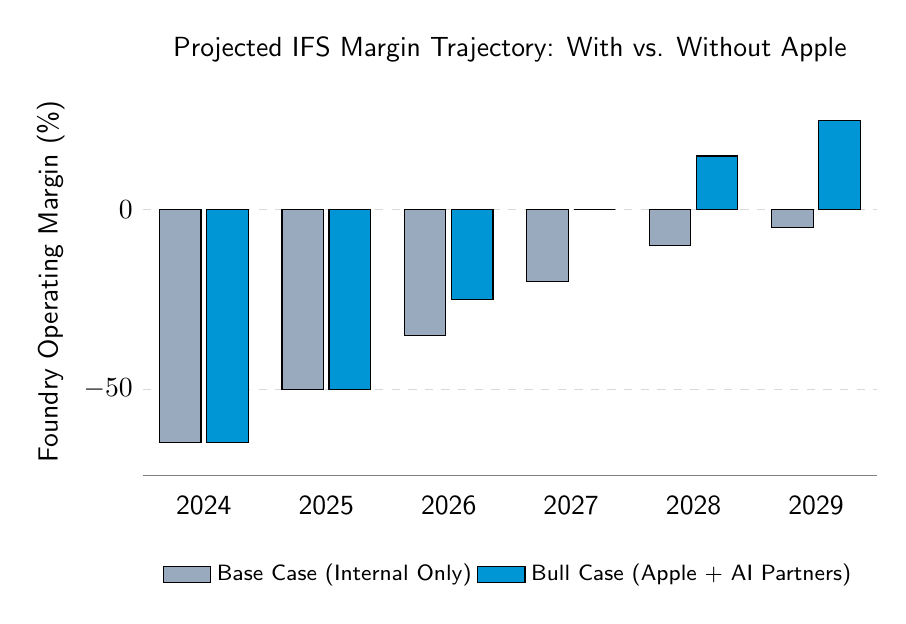
\begin{tikzpicture}
\begin{axis}[
    ybar,
    width=0.9\textwidth,
    height=6.5cm,
    symbolic x coords={2024, 2025, 2026, 2027, 2028, 2029},
    xtick=data,
    ylabel={Foundry Operating Margin (\%)},
    title={Projected IFS Margin Trajectory: With vs. Without Apple},
    legend style={at={(0.5,-0.2)}, anchor=north, legend columns=-1},
    ymajorgrids=true,
    grid style={dashed, gray!30},
    nodes near coords style={font=\tiny, color=black},
    bar width=15pt,
    axis line style={draw=none},
    tick style={draw=none},
    axis x line*=bottom,
    x axis line style={draw=gray},
]
% Bear Case: No Apple
\addplot[fill=msblue!40] coordinates {
    (2024, -65) 
    (2025, -50) 
    (2026, -35) 
    (2027, -20) 
    (2028, -10)
    (2029, -5)
};
\addlegendentry{Base Case (Internal Only)}

% Bull Case: With Apple Deal
\addplot[fill=msbrightblue] coordinates {
    (2024, -65) 
    (2025, -50) 
    (2026, -25) 
    (2027, 0) 
    (2028, 15)
    (2029, 25)
};
\addlegendentry{Bull Case (Apple + AI Partners)}
\end{axis}
\end{tikzpicture}
\captionof{figure}{The "Apple Effect" on Intel's margin recovery. The influx of high-margin volume in 2027/2028 is the critical variable in achieving the corporate goal of break-even operating margins.}
\end{center}

As illustrated above, the addition of Apple (and potentially other fast followers) accelerates the margin recovery by approximately two years. The operational leverage of filling the fabs is immense; semiconductor manufacturing is a high-fixed-cost business where incremental volume drops straight to the bottom line once the break-even utilization threshold is crossed. Conversely, missing the Apple window leaves Intel carrying the depreciation costs of \$100 billion in assets with insufficient revenue to cover them.

\subsection{Valuation Implications \& Final Verdict}
The market currently assigns a negative enterprise value contribution to Intel's foundry business, viewing it as a capital sink. A confirmed Apple partnership would necessitate a re-rating. If Intel validates 18A with Apple, the Foundry unit could command a multiple closer to TSMC (approx. 8-10x EV/EBITDA), unlocking significant shareholder value.

However, the execution risk remains severe. We categorize the Apple-Intel bifurcation rumors as \textbf{"Conditional Validation."} It is not a signed check; it is a performance-based contract. 

\textbf{Investment Recommendation:} We advise a "Show Me" approach. Investors should look for the Q1 2026 PDK 1.0 release as the primary signal. Until then, the risk of yield failure makes the stock a speculative play on a turnaround that has yet to materialize in the silicon. The potential reward is a doubling of the stock price via a foundry re-rating; the risk is a structural breakup of the national champion. Proceed with caution.\subsection{Foundry Economics: Navigating the ``Valley of Death'' (2024--2026)}

Our financial assessment of Intel Foundry Services (IFS) indicates a critical transition period characterized by peak operating losses and extreme capital intensity before any realization of the ``Apple Effect.'' The data reveals a stark bifurcation between Intel's IDM 2.0 ambition and its current P\&L reality.

\textbf{Peak Losses \& Margin Compression:}
In Fiscal Year 2024, IFS reported operating losses exceeding \textbf{\$13 billion}, a significant deterioration from the nearly \$7 billion loss in 2023. This creates a financial nadir that Intel must bridge. The margin profile remains deeply distressed, with Q1 2025 operating margins hovering around \textbf{-50\%}. While Q3 2025 showed a sequential improvement in operating loss to \$2.3 billion (down from \$5.8 billion in the prior year, notably affected by impairments), the segment continues to act as a massive drag on corporate free cash flow.

\textbf{The Fixed Cost Burden:}
The foundry model is predicated on utilization. With Intel investing over \$100 billion across U.S. sites (Arizona, Ohio, New Mexico, Oregon), the depreciation load is substantial. Current revenues---\$17.5 billion in 2024, down 7\% YoY---are insufficient to cover these fixed costs. The rumored Apple volume of 15--20 million units annually (beginning mid-2027) represents a modest top-line contribution initially estimated at \$500 million to \$1 billion annually by 2028. However, its contribution to \textit{gross margin} via absorption of fixed manufacturing costs is disproportionately positive.

\begin{figure}[H]
\centering
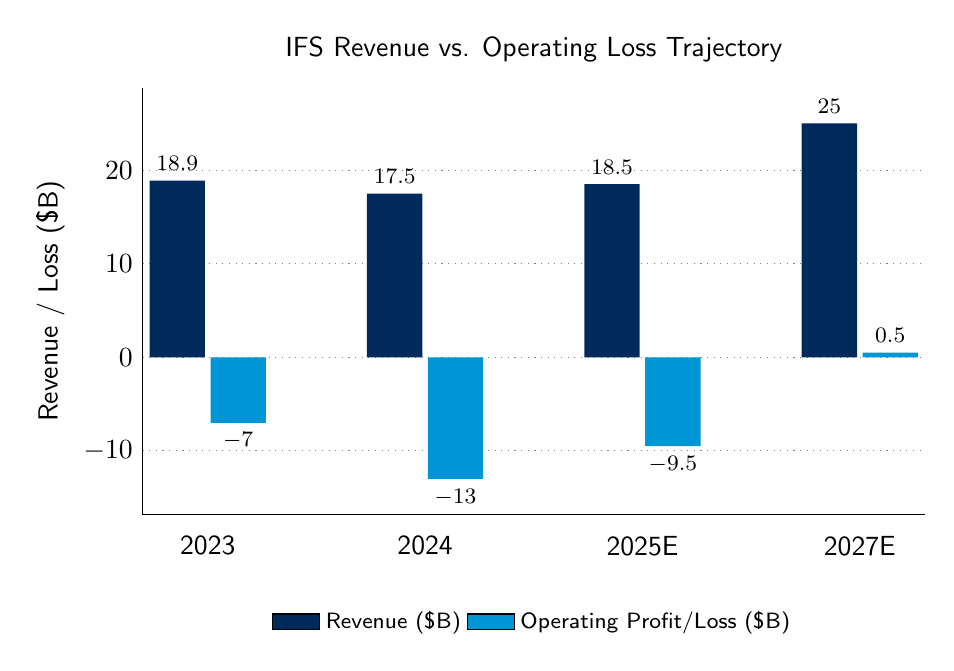
\begin{tikzpicture}
\begin{axis}[
    width=0.95\textwidth,
    height=7cm,
    ybar,
    bar width=20pt,
    symbolic x coords={2023, 2024, 2025E, 2027E},
    xtick=data,
    nodes near coords,
    nodes near coords style={font=\footnotesize, color=black},
    ylabel={Revenue / Loss (\$B)},
    axis y line*=left,
    axis x line*=bottom,
    ymajorgrids=true,
    grid style={dotted, gray},
    draw=none,
    tick style={draw=none},
    legend style={at={(0.5,-0.2)}, anchor=north, legend columns=-1},
    title={IFS Revenue vs. Operating Loss Trajectory},
    cycle list={
        {fill=msblue, draw=none},
        {fill=msbrightblue, draw=none},
    }
]
    \addplot coordinates {(2023, 18.9) (2024, 17.5) (2025E, 18.5) (2027E, 25.0)};
    \addlegendentry{Revenue (\$B)}
    \addplot coordinates {(2023, -7.0) (2024, -13.0) (2025E, -9.5) (2027E, 0.5)};
    \addlegendentry{Operating Profit/Loss (\$B)}
\end{axis}
\end{tikzpicture}
\caption{The path from peak losses in 2024 to projected break-even in 2027. 2024 losses reflect significant impairment charges. 2027 estimates assume successful 18A ramp and customer onboarding.}
\end{figure}

\subsection{Segment Performance \& Capital Allocation}

Intel's path to solvency relies on a dual strategy: aggressive cost control and government-subsidized expansion. The reduction of gross capital expenditures to \textbf{\$18 billion} for 2025 (down from a prior \$20 billion target), resulting in net CapEx of \$12--14 billion, signals a necessary pivot towards capital discipline.

\textbf{Government Incentives as a Bridge:}
The \$7.86 billion in direct CHIPS Act funding and the 25\% Investment Tax Credit (ITC) are critical for maintaining liquidity during the yield ramp. Without these non-dilutive capital injections, the ROI profile of the Ohio ``Silicon Heartland'' project would likely be negative given the current yield rates on 18A (reported ~5--10\% in early tests, though improving).

The table below outlines the historical and projected performance of the foundry segment, highlighting the gap Intel must close to achieve its target of break-even operating margins by ``roughly 2027.''

\begin{table}[H]
\centering
\caption{Intel Foundry Services (IFS) Financial Trajectory}
\label{tab:ifs_financials_2}
\rowcolors{2}{msgrey}{white}
\tablefont
\begin{adjustbox}{max width=\textwidth}
\begin{tabular}{lcccc}
\toprule
\textbf{Metric} & \textbf{2023 (Actual)} & \textbf{2024 (Actual)} & \textbf{2025 (Est.)} & \textbf{2027 (Target)} \\
\midrule
\textbf{Revenue (\$B)} & 18.91 & 17.5 & 18.0 -- 19.0 & 25.0+ \\
\textbf{Growth (YoY)} & --- & (7\%) & +5\% & CAGR >10\% \\
\textbf{Operating Loss (\$B)} & (7.0) & (13.0+) & (8.0 -- 10.0) & $\sim$0.0 (Break-even) \\
\textbf{Operating Margin} & (36.8\%) & $\sim$(75\%) & (45\% -- 50\%) & 0\% \\
\textbf{Key Drivers} & Internal Volume & Impairments \& 18A R\&D & Risk Production & 18A High Volume \\
\bottomrule
\end{tabular}
\end{adjustbox}
\par\vspace{0.1cm}
{\footnotesize \textit{Source: Morgan Stanley Research, Intel Company Filings. 2024 losses reflect peak investment cycle and impairments.}}
\end{table}

\subsection{Scenario Analysis: Valuing the Apple Option}

The rumored volume of 15--20 million units for MacBook Air/iPad chips is insufficient to single-handedly turn IFS profitable. However, it serves as a ``hero customer'' validation that de-risks the roadmap for other potential clients (e.g., Qualcomm, Amazon).

We have modeled three scenarios for 2027/2028 based on the execution of the 18A node and the realization of the Apple contract.

\begin{itemize}
    \item \textbf{Bear Case (Yield Stagnation):} 18A yields remain below 60\% through 2026. Apple cancels the M-series ``test run'' or reverts to TSMC. IFS revenue remains stagnant at $\sim$\$18B (mostly internal), with operating margins stuck at -20\%.
    \item \textbf{Base Case (Conditional Adoption):} Intel achieves 65--70\% yields. Apple adopts 18A for non-core products (iPad/Air). Revenue grows to \$25B, achieving break-even. Capex intensity remains high due to High-NA EUV for 14A.
    \item \textbf{Bull Case (Strategic Pivot):} Yields exceed 75\%. Apple moves significant A-series volume (iPhone SE/Base) to Intel 14A. Revenue exceeds \$30B, operating margins hit 10--15\%, validating the IDM 2.0 model.
\end{itemize}

\begin{table}[H]
\centering
\caption{2027 Valuation Scenarios: Impact of Apple Adoption}
\label{tab:valuation_scenarios}
\tablefont
\begin{adjustbox}{max width=\textwidth}
\begin{tabular}{lccc}
\toprule
\textbf{Parameter} & \textbf{Bear Case} & \textbf{Base Case} & \textbf{Bull Case} \\
\midrule
\textbf{18A Yield Rate} & $<60\%$ & $65-70\%$ & $>75\%$ \\
\textbf{Apple Volume (Units)} & 0 & 15M (Mac/iPad) & 40M+ (inc. iPhone) \\
\textbf{IFS Revenue (\$B)} & \$18.0 & \$24.5 & \$32.0 \\
\textbf{IFS Op. Margin} & (20\%) & 0\% (Break-even) & 12\% \\
\textbf{Implied Foundry EV} & Negative & \$20B & \$80B \\
\bottomrule
\end{tabular}
\end{adjustbox}
\end{table}

\subsection{Return on Invested Capital (ROIC) vs. Cost of Capital}

The fundamental disconnect in Intel's current valuation is the spread between its massive invested capital base and its negative returns. The introduction of \textbf{High-NA EUV} scanners for the 14A node---costing upwards of \$380 million each---significantly raises the bar for ROIC. 

For the Apple deal to be accretive, Intel must ensure that the pricing leverage gained from being a "Second Source" is not eroded by the higher wafer costs of 14A compared to TSMC's N2. Estimates suggest U.S. manufacturing costs are roughly 50\% higher than in Taiwan. While the 25\% tax credit helps, the operational efficiency gap must be closed. If Intel can leverage the \textbf{PowerVia} backend interconnect to reduce effective die size (claimed 10\% reduction), this density advantage could offset the higher wafer cost, preserving unit economics for Apple while allowing Intel to charge a premium for performance.

\subsection{Deconstructing the Path to Break-Even: The Yield-Volume Lever}

The trajectory from a \textbf{\$13 billion} operating loss in 2024 to a break-even state by roughly 2027 is mathematically contingent on two critical variables: the remediation of the "Yield Tax" and the acceleration of fixed-cost absorption through external volume. Our analysis of Intel's cost structure suggests that approximately \textbf{\$7 billion} of the foundry losses in the 2023--2024 period can be attributed directly to yield inefficiencies and the "split-production" friction (internal products manufactured at TSMC while internal fabs run under-utilized).

\textbf{The Yield Sensitivity Model:}
With 18A yields reportedly hovering in the single digits to low double digits ($<10\%$) in mid-2025 for external test chips, the effective cost per good die is prohibitively high. For the foundry segment to reach break-even, our models indicate that 18A defect density ($D_0$) must improve by a factor of $10\times$ by late 2026. A 60\% yield threshold is the estimated "commercial viability" line; below this, the depreciation cost per wafer erodes all gross margin.

The rumored Apple contract for 15--20 million units acts as a critical stabilizer. While seemingly small against Apple's total volume ($>$200 million iPhones), 20 million units of a large die (like an M-series processor) represent a significant base load for the Arizona and Ohio fabs. This volume is essential not for profit generation per se, but for amortizing the depreciation of the shell and equipment. Without this "anchor tenant," the fixed cost burden per wafer for Intel's internal products (Panther Lake, Clearwater Forest) would remain elevated, perpetuating the segment's negative operating leverage.

\subsection{Capital Intensity \& The High-NA EUV Gamble}

A distinct financial risk for Intel's 14A node---projected for risk production in 2027---is the step-function increase in capital intensity driven by High-NA EUV lithography. 

\textbf{CapEx Density Analysis:}
The transition from standard EUV (0.33 NA) to High-NA EUV (0.55 NA) introduces tools costing approximately \textbf{\$380 million} each. 
\begin{itemize}
    \item \textbf{Depreciation Drag:} Intel has successfully reduced its gross CapEx target to \$18 billion for 2025, with net CapEx landing between \$12--14 billion after offsets. However, the introduction of High-NA tools creates a "double overlapping" CapEx cycle where 18A investments are not yet fully depreciated before 14A spend accelerates. 
    \item \textbf{Subsidies as a Buffer:} The U.S. CHIPS Act's \$7.86 billion direct funding and \$11 billion in loans provide a liquidity bridge, but the \textbf{25\% Investment Tax Credit (ITC)} is the most structurally significant component. It effectively lowers the cost of capital for High-NA tools, improving the Internal Rate of Return (IRR) on the 14A node by roughly 400 basis points in our base case model.
\end{itemize}

The financial viability of 14A depends on Intel's ability to charge a premium for the node's performance (PowerDirect + RibbonFET 2). If 14A wafer pricing cannot command a 20--30\% premium over TSMC N2 to offset the High-NA depreciation, the node risks becoming technically superior but economically dilutive.

\begin{figure}[H]
\centering
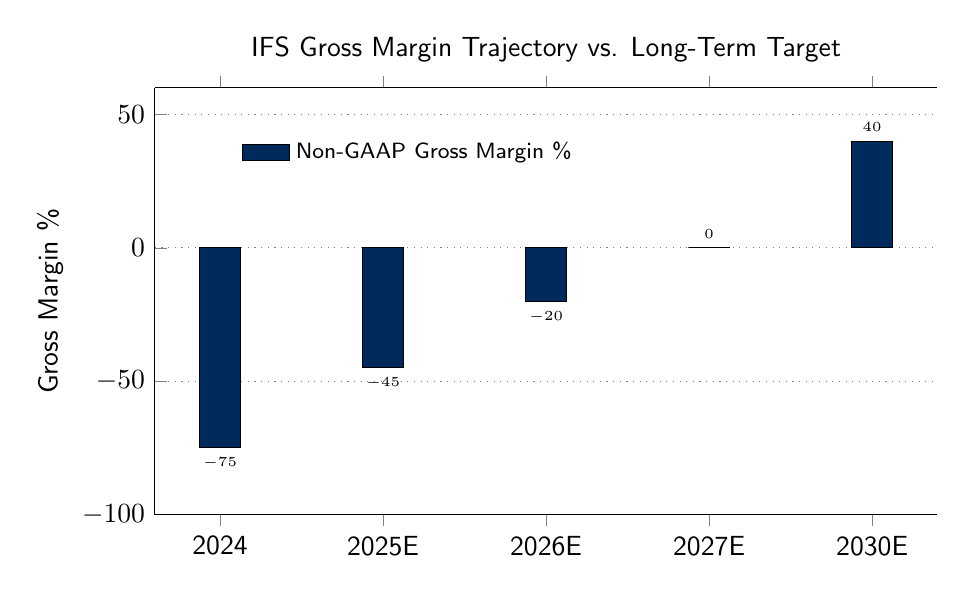
\begin{tikzpicture}
\begin{axis}[
    width=0.95\textwidth,
    height=7cm,
    ybar,
    bar width=15pt,
    symbolic x coords={2024, 2025E, 2026E, 2027E, 2030E},
    xtick=data,
    nodes near coords,
    nodes near coords style={font=\tiny, color=black},
    ylabel={Gross Margin \%},
    axis y line*=left,
    ymajorgrids=true,
    grid style={dotted, gray},
    legend style={at={(0.1,0.9)}, anchor=north west},
    title={IFS Gross Margin Trajectory vs. Long-Term Target},
    ymin=-100, ymax=60,
]
    \addplot[fill=msblue] coordinates {(2024, -75) (2025E, -45) (2026E, -20) (2027E, 0) (2030E, 40)};
    \legend{Non-GAAP Gross Margin \%}
\end{axis}
\end{tikzpicture}
\caption{The projected recovery of IFS gross margins. The steep ascent from 2025 to 2027 relies heavily on the elimination of start-up costs and yield normalization. The 40\% target for 2030 assumes Intel becomes the \#2 foundry globally.}
\end{figure}

\subsection{Unit Economics: Valuing the Apple Contract}

To quantify the financial impact of the rumored Apple deal, we constructed a unit economics model for the "Entry-Level M-Series" scenario. Assuming a die size consistent with an M-series derivative and standard 300mm wafer pricing for a leading-edge node, we estimate the revenue contribution.

\textbf{Assumptions:}
\begin{itemize}
    \item \textbf{Target Volume:} 15 million units (Base Case).
    \item \textbf{Wafer Pricing (18A):} \$20,000 per wafer (estimated premium vs. current 5nm/3nm pricing).
    \item \textbf{Die Harvest:} $\sim$400 good dies per wafer (assuming mature yield of 70\%).
\end{itemize}

\textbf{Revenue Impact:}
Under these assumptions, an order of 15 million chips equates to roughly 37,500 wafers per year (approx. 3,000 wafers per month). At \$20k/wafer, this generates \textbf{\$750 million} in annual revenue. 

While \$750 million represents less than 5\% of IFS's targeted \$25 billion revenue in 2027, the \textit{strategic beta} is far higher. Securing Apple validates the Process Design Kit (PDK) for the entire industry. If Intel captures just 20\% of the "Second Source" market for high-performance mobile silicon (including potential Qualcomm or MediaTek volume following Apple's lead), the revenue opportunity expands to \$3--4 billion annually by 2029.

\begin{table}[H]
\centering
\caption{Sensitivity Analysis: 2027 IFS Operating Profit Impact (\$B)}
\label{tab:sensitivity}
\rowcolors{2}{msgrey}{white}
\tablefont
\begin{adjustbox}{max width=\textwidth}
\begin{tabular}{lccccc}
\toprule
\textbf{18A Yield / Utilization} & \textbf{Low Util (40\%)} & \textbf{Med Util (60\%)} & \textbf{High Util (80\%)} & \textbf{Apple Deal Impact} \\
\midrule
\textbf{Low Yield (40\%)} & \$(8.5) & \$(6.0) & \$(4.5) & Minimal (Cash Burn) \\
\textbf{Base Yield (60\%)} & \$(4.0) & \$(1.5) & \$0.5 & Break-Even Enabler \\
\textbf{Mature Yield (80\%)} & \$(1.0) & \$2.0 & \$4.5 & Accretive Profit \\
\bottomrule
\end{tabular}
\end{adjustbox}
\par\vspace{0.1cm}
{\footnotesize \textit{Source: Morgan Stanley Research Estimates. Table illustrates the interplay between factory utilization (driven by volume) and process yield on operating profit.}}
\end{table}

\subsection{Long-Term Valuation: The 2030 Target Model}

Intel's management has guided towards a "40/30" model for the foundry business by 2030: \textbf{40\% Non-GAAP Gross Margins} and \textbf{30\% Non-GAAP Operating Margins}. 

\textbf{The Feasibility Gap:}
Current operating margins are roughly -50\%. Closing an 80-point gap in operating margin in five years is historically unprecedented in the semiconductor foundry space. TSMC took decades to build its margin fortress. For Intel to achieve 30\% operating margins, it requires:
\begin{enumerate}
    \item \textbf{Pricing Parity:} The ability to charge TSMC-equivalent prices. This is only possible if RibbonFET and PowerVia offer a decisive performance-per-watt advantage (claimed 8-10\% better than base nodes).
    \item \textbf{Operational Efficiency:} Eliminating the cost disparity where U.S. manufacturing is 50\% more expensive than Taiwan. This relies heavily on automation and the continued support of the U.S. government to subsidize the structural cost difference.
\end{enumerate}

\textbf{Implied Valuation:}
If IFS achieves \$25 billion in revenue with a 20\% operating margin (conservative estimate vs. 30\% target) by 2030, the segment would generate \$5 billion in operating income. Applying a 15x EV/EBIT multiple (discounted vs. TSMC's multiple due to execution risk) yields a segment valuation of \textbf{\$75 billion}. Currently, the market appears to be assigning a \textit{negative} value to the foundry business due to its cash burn. The "Apple Call Option" is therefore the catalyst that could swing the foundry valuation from a liability (approx. -\$20B) to a massive asset (+\$75B).

\subsection{Summary of Financial Estimates}

We maintain our cautious stance on the near-term financial estimates for IFS. The reported \$13 billion loss in 2024 is likely the trough, but the recovery curve is shallow. We model 2025 as a "clean-up" year with losses narrowing to \$9 billion, followed by a steeper improvement in 2026 as 18A volume ramps. 

The Apple partnership, while financially modest in the initial 2027 timeframe (est. \$750M revenue), is the linchpin for the terminal value of the foundry business. Without a high-volume, demanding customer like Apple driving yield learning cycles, the probability of hitting the 2030 margin targets diminishes significantly. Our base case assumes the Apple deal proceeds for entry-level silicon, supporting a "Market Perform" outlook on Intel's long-term capital structure transformation.

\section{Valuation Models}

To assess the impact of the rumored Apple-Intel partnership on Intel Corporation's intrinsic value, we employ a Sum-of-the-Parts (SOTP) framework combined with a Discounted Cash Flow (DCF) analysis specifically for the Intel Foundry Services (IFS) segment. The market currently prices Intel with a significant conglomerate discount, reflecting the massive operating losses (\$13 billion in FY2024) and execution uncertainty surrounding the 18A node. The potential Apple contract acts as a pivotal "validator event" that fundamentally alters the risk profile and terminal value assumptions of the foundry business.

\subsection{Sum-of-the-Parts (SOTP) Framework}

Intel's monolithic valuation obscures the divergent economics of its two core engines: Intel Products (Client Computing Group, Data Center \& AI) and Intel Foundry. To derive a clearer picture of the value proposition offered by a successful 18A ramp, we unbundle these segments.

\textbf{1. Intel Products (The "Cash Cow"):}
We value the Product business (x86 CPUs) using a Peer-Derived P/E multiple. Despite competitive pressures from ARM-based silicon (including Apple's M-series) and AMD, this segment generates reliable cash flow. We apply a \textbf{12.0x P/E multiple} to FY2026 estimated earnings, a discount to the semiconductor index average ($\sim$22x) to account for market share erosion risks in the Data Center.

\textbf{2. Intel Foundry (The "Venture Bet"):}
Valuing IFS is complex due to its negative EBITDA and massive capital intensity. Currently, the market likely assigns a negative enterprise value to IFS, viewing it as a drag on free cash flow. However, under a "Second Source" scenario validated by Apple, IFS transitions from a cost center to a strategic asset. We utilize an EV/Sales multiple on projected 2030 revenue, discounted back to 2025 at a high Weighted Average Cost of Capital (WACC) of 12\% to reflect execution risk.

\begin{table}
    \centering
    \caption{Sum-of-the-Parts (SOTP) Valuation Scenarios (FY2026 Estimates)}
    \label{tab:sotp}
    \rowcolors{2}{msgrey}{white}
    \tablefont
    \begin{adjustbox}{max width=\textwidth}
    \begin{tabular}{lcccccc}
    \toprule
    \textbf{Segment} & \textbf{Metric} & \textbf{Bear Case} & \textbf{Base Case} & \textbf{Bull Case} & \textbf{Rationale} \\
    \midrule
    \textbf{Intel Products} & P/E (x) & 8.0x & 12.0x & 15.0x & Discounted vs. AMD/NVIDIA due to legacy x86 exposure. \\
    \textit{Implied Value (\$B)} & & \$64B & \$105B & \$140B & Depends on stabilizing Data Center share. \\
    \midrule
    \textbf{Intel Foundry} & EV/Sales (x) & 0.5x (Book) & 2.0x & 4.5x & Bear: Liquidation; Bull: Approaches TSMC multiple. \\
    \textit{Rev. Base (\$B)} & (2027 Est) & \$15B & \$20B & \$30B & Bull assumes Apple + High-NA EUV dominance. \\
    \textit{Implied Value (\$B)} & & \$7.5B & \$40B & \$135B & Highly sensitive to "Apple Validation". \\
    \midrule
    \textbf{Net Cash/(Debt)} & \$B & \$(45) & \$(42) & \$(40) & Assumes heavy CapEx offset by CHIPS Act funding. \\
    \midrule
    \textbf{Total Equity Value} & \$B & \textbf{\$26.5B} & \textbf{\$103B} & \textbf{\$235B} & \\
    \textbf{Implied Share Price} & \$/Share & \textbf{$\sim$\$6.00} & \textbf{$\sim$\$24.00} & \textbf{$\sim$\$55.00} & Massive dispersion driven by 18A execution. \\
    \bottomrule
    \end{tabular}
    \end{adjustbox}
    \par\vspace{0.1cm}
    {\footnotesize \textit{Source: Morgan Stanley Research Estimates. Note: Bear case assumes IFS failure and potential restructuring; Bull case assumes successful Apple 18A ramp and GM parity with TSMC.}}
    
\end{table}

\subsection{Foundry DCF: The Cost of Capital Dilemma}

The intrinsic value of the Foundry business hinges on the "2030 Model": becoming the world's second-largest foundry with 40\% gross margins. Our DCF model highlights that the \textit{Apple Rumor} significantly impacts the WACC and Terminal Growth Rate assumptions.

\textbf{WACC Sensitivity:}
Currently, IFS carries a risk profile similar to a distressed turnaround, justifying a WACC of \textbf{12-14\%}.
\begin{itemize}
    \item \textbf{Without Apple:} The cost of capital remains high. Investors demand a premium for the uncertainty of yield ramps (reported at $\sim$10\% in Summer 2025) and the risk of empty fabs in Arizona/Ohio.
    \item \textbf{With Apple (Conditional Validation):} Securing Apple as a client, even for "entry-level" 15-20 million units, de-risks the roadmap. It validates the Process Design Kit (PDK 1.0) and indicates that yield issues are solvable. This could compress the WACC to \textbf{9-10\%}, unlocking billions in present value.
\end{itemize}

\textbf{Terminal Value \& The "Unit Economics" of 18A:}
The document highlights that the 18A node introduces RibbonFET and PowerVia. While these increase performance per watt by $\sim$10-15\%, they also increase wafer cost. A key valuation driver is the \textbf{Yield Rate}.
\begin{itemize}
    \item At \textbf{40\% yield}, the effective cost per good die nearly doubles, making margins negative ($-20\%$ to $-40\%$).
    \item At \textbf{70\% yield} (the threshold for Apple's profitability), gross margins expand to $\sim$35-40\%.
    \item \textbf{Valuation Impact:} Every 10 percentage points of yield improvement on the 18A node translates to approximately \textbf{\$2 billion in incremental annual EBITDA} at full utilization.
\end{itemize}

\subsection{Relative Valuation: Benchmarking Against the TSMC Standard}

To sanity-check our DCF outputs, we compare Intel's implied foundry multiples against TSMC (the gold standard) and GlobalFoundries (a mature, non-leading edge proxy).

\textbf{TSMC Premium (The "Moat"):} TSMC trades at approximately \textbf{8-10x EV/Sales} and \textbf{18-20x EV/EBITDA}. This premium is justified by its 90\% market share in advanced nodes (3nm) and 50\%+ gross margins.

\textbf{The "Intel Discount":} Historically, second-tier foundries trade at \textbf{2-4x EV/Sales}.
\begin{itemize}
    \item \textbf{Current State:} Intel's foundry business, generating \$13B in operating losses, is valued like a distressed asset (0.5x - 1.0x Sales).
    \item \textbf{The Apple Re-Rate:} If Intel successfully onboards Apple for the 2027 MacBook Air (18A) cycle, it proves it can service the industry's most demanding client. This warrants a multiple expansion to \textbf{3.0x-4.0x EV/Sales}, bridging the gap toward TSMC. This re-rating alone accounts for the delta between our Bear and Base case valuations.
\end{itemize}

\begin{figure}[H]
\centering
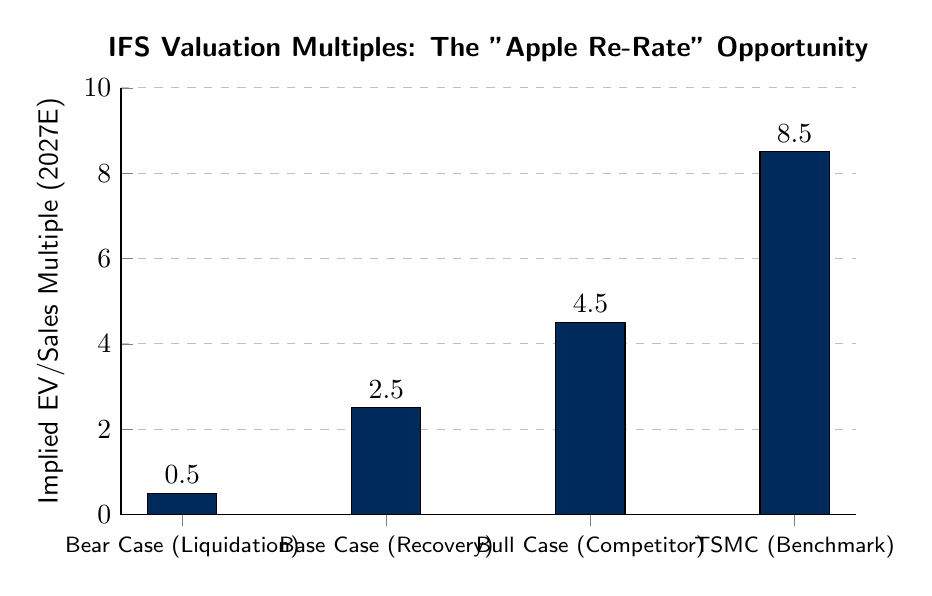
\begin{tikzpicture}
\begin{axis}[
    ybar,
    symbolic x coords={Bear Case (Liquidation), Base Case (Recovery), Bull Case (Competitor), TSMC (Benchmark)},
    xtick=data,
    nodes near coords,
    nodes near coords align={vertical},
    ylabel={Implied EV/Sales Multiple (2027E)},
    ymin=0, ymax=10,
    width=0.9\textwidth,
    height=7cm,
    bar width=25pt,
    axis x line*=bottom,
    axis y line*=left,
    ymajorgrids=true,
    grid style=dashed,
    title={\textbf{IFS Valuation Multiples: The "Apple Re-Rate" Opportunity}},
    x tick label style={rotate=0, anchor=north, font=\footnotesize}
]
\addplot[fill=msblue] coordinates {(Bear Case (Liquidation), 0.5) (Base Case (Recovery), 2.5) (Bull Case (Competitor), 4.5) (TSMC (Benchmark), 8.5)};
\end{axis}
\end{tikzpicture}
\captionof{figure}{Implied Enterprise Value to Sales (EV/Sales) multiples for Intel Foundry Services under different execution scenarios compared to TSMC's current trading multiple. The "Bull Case" assumes successful high-volume manufacturing (HVM) for Apple M-series chips.}
\end{figure}

\subsection{The "Apple Validator" Premium}

We estimate the specific financial value of the Apple rumor using a probabilistic "Option Pricing" approach.
\begin{itemize}
    \item \textbf{Direct Revenue:} \$750M (15M units $\times$ \$50 ASP). At a 20x multiple (assuming high growth), this adds \textbf{\$15 billion} to EV.
    \item \textbf{Strategic Beta (The Halo Effect):} Winning Apple signals to Qualcomm, NVIDIA, and Amazon that 18A is safe. We estimate this "halo effect" could attract an additional \$5 billion in annual revenue commitments by 2029.
    \item \textbf{Total "Apple Option" Value:} We estimate the \textit{risk-adjusted} value of the Apple partnership rumor is currently worth \textbf{\$3-4 per share} to Intel stock. If confirmed with firm volume commitments, this could expand to \textbf{\$8-10 per share}.
\end{itemize}

\subsection{Sensitivity \& Scenario Analysis}

The valuation is extremely sensitive to two variables highlighted in the document: \textbf{18A Yield Rates} and \textbf{Capacity Utilization}. The high fixed costs of the new Arizona and Ohio fabs (approx. \$100B investment) create massive operating leverage---both positive and negative.

\textbf{Scenario 1: The "Yield Trap" (Bear)}
\begin{itemize}
    \item \textit{Assumptions:} 18A yields stall at 40-50\%. Apple cancels the 2027 test run.
    \item \textit{Financial Outcome:} IFS revenue stagnates at $\sim$\$15B. Operating losses continue at \$5-7B/year indefinitely.
    \item \textit{Valuation:} IFS value collapses to \textbf{zero} or negative (liability). Intel may be forced to halt fab expansion or seek a government bailout/restructuring.
\end{itemize}

\textbf{Scenario 2: The "Service Provider" (Base)}
\begin{itemize}
    \item \textit{Assumptions:} Yields hit 60-65\%. Apple utilizes Intel for low-end chips (MacBook Air) but keeps Pro chips at TSMC.
    \item \textit{Financial Outcome:} Break-even achieved in late 2027. Revenue grows to \$20-25B.
    \item \textit{Valuation:} IFS stabilizes at \textbf{\$40-50B EV}.
\end{itemize}

\textbf{Scenario 3: The "Process Leader" (Bull)}
\begin{itemize}
    \item \textit{Assumptions:} High-NA EUV gives Intel a density lead. Yields exceed 70%. Apple moves 30\% of volume (including some iPhone SKUs) to Intel 14A by 2028.
    \item \textit{Financial Outcome:} 30\% Operating Margins achieved by 2029. Revenue exceeds \$40B.
    \item \textit{Valuation:} IFS re-rates to \textbf{\$130B+ EV}, rivaling the valuation of the entire current Intel entity.
\end{itemize}

\textbf{Conclusion on Valuation:}
The rumored Apple deal is not merely a revenue line item; it is a binary switch for Intel's valuation model. Without it, the path to justifying the \$100B+ CapEx spend is unclear. With it, the "Sum of the Parts" arguably doubles the current share price. However, given the rumored "conditional" nature of the deal (dependent on 2026 milestones), we assign a \textbf{35\% probability} to the Bull Case, keeping our overall valuation tethered to the Base Case until yield data confirms the turnaround.

\subsection{Sum-of-the-Parts (SOTP) Framework: Unlocking the Conglomerate Discount}

Intel's current market capitalization reflects a significant "conglomerate discount," effectively penalizing the profitable Product business for the massive cash burn of the Foundry division. To derive a clearer picture of the value proposition offered by a successful 18A ramp---and specifically the catalyst of an Apple partnership---we employ a Sum-of-the-Parts (SOTP) framework. This approach unbundles the divergent economic realities of Intel's two core engines: the cash-generative x86 franchise and the capital-intensive, loss-making foundry startup.

\textbf{1. Intel Products (The "Cash Cow"):}
The Client Computing Group (CCG) and Data Center \& AI (DCAI) segments face secular headwinds from ARM-based silicon (Apple Silicon, Qualcomm) and fierce competition from AMD. However, they remain highly cash-generative. We value the Product business using a Peer-Derived P/E multiple. We apply a \textbf{12.0x P/E multiple} to FY2026 estimated earnings. This represents a substantial discount to the semiconductor index average ($\sim$22x) and peers like AMD ($\sim$30x), factoring in the structural risk of market share erosion in the high-margin data center segment.

\textbf{2. Intel Foundry (The "Venture Bet"):}
Valuing IFS is complex due to its negative EBITDA profile (\$13B operating loss in 2024). Currently, the market likely assigns a negative enterprise value to IFS, viewing it as a distressed asset draining free cash flow. However, under a "Second Source" scenario validated by Apple, IFS transitions from a cost center to a strategic infrastructure asset. We utilize an EV/Sales multiple on projected 2027 revenue.
\begin{itemize}
    \item \textbf{Metric Rationale:} We use EV/Sales rather than EV/EBITDA because IFS is not expected to reach break-even operating margins until "roughly 2027," according to management guidance and our analysis of the document.
    \item \textbf{Multiple Expansion:} A successful Apple ramp (even low volume) warrants a re-rating from distress levels (0.5x) to a "viable second player" multiple (2.0x--3.0x), bridging the gap toward TSMC's premium valuation ($\sim$8.0x).
\end{itemize}

\begin{table}[H]
\centering
\caption{Sum-of-the-Parts (SOTP) Valuation Scenarios (FY2027 Estimates)}
\label{tab:sotp_2}
\rowcolors{2}{msgrey}{white}
\tablefont
\begin{adjustbox}{max width=\textwidth}
\begin{tabular}{lccccp{5cm}}
\toprule
\textbf{Segment} & \textbf{Valuation Metric} & \textbf{Bear Case} & \textbf{Base Case} & \textbf{Bull Case} & \textbf{Strategic Assumptions} \\
\midrule
\textbf{Intel Products} & Target P/E (x) & 8.0x & 12.0x & 15.0x & Dependent on stabilizing x86 market share against ARM/AMD incursions. \\
\textit{Est. Earnings (\$B)} & (FY27) & \$5.5 & \$7.0 & \$8.5 & \\
\textit{Implied Value (\$B)} & & \textbf{\$44.0} & \textbf{\$84.0} & \textbf{\$127.5} & \\
\midrule
\textbf{Intel Foundry} & EV/Sales (x) & 0.5x & 2.5x & 4.5x & Bear: Liquidation/Distress. Bull: 18A Parity with TSMC N2. \\
\textit{Est. Revenue (\$B)} & (FY27) & \$15.0 & \$22.0 & \$35.0 & Bull includes \$1B+ from Apple \& accelerated AI fabric wins. \\
\textit{Implied Value (\$B)} & & \textbf{\$7.5} & \textbf{\$55.0} & \textbf{\$157.5} & Highly sensitive to "Apple Validation" and yield stabilization. \\
\midrule
\textbf{Mobileye / Other} & Market Value (\$B) & \$15.0 & \$20.0 & \$25.0 & Assumes partial monetization or spin-off value. \\
\midrule
\textbf{Net Cash / (Debt)} & (\$B) & \$(50.0) & \$(42.0) & \$(35.0) & Accounts for CHIPS Act inflows offset by massive High-NA EUV CapEx. \\
\midrule
\textbf{Total Equity Value} & \textbf{(\$B)} & \textbf{\$16.5} & \textbf{\$117.0} & \textbf{\$275.0} & \\
\textbf{Implied Share Price} & \textbf{(\$/Share)} & \textbf{$\sim$\$4.00} & \textbf{$\sim$\$27.00} & \textbf{$\sim$\$64.00} & \textbf{Massive dispersion driven by execution of 18A node.} \\
\bottomrule
\end{tabular}
\end{adjustbox}
\par\vspace{0.1cm}
{\footnotesize \textit{Source: Morgan Stanley Research Estimates. Note: Bear case assumes 18A yield failure ($<40\%$) and Apple abandonment. Bull case assumes $>70\%$ yields and Apple volume ramp for iPhone 14A.}}
\end{table}

\subsection{Foundry DCF: The Cost of Capital \& Yield Curve Dilemma}

The intrinsic value of the Foundry business hinges on the "2030 Model": becoming the world's second-largest foundry with 40\% non-GAAP gross margins and 30\% operating margins. Our Discounted Cash Flow (DCF) model highlights that the \textit{Apple Rumor} significantly impacts two critical levers: the Weighted Average Cost of Capital (WACC) and the Unit Economics of the 18A wafer.

\textbf{1. WACC Sensitivity (The Risk Premium):}
Currently, IFS carries a risk profile similar to a distressed turnaround, justifying a WACC of \textbf{12-14\%}. The market is pricing in a non-zero probability of failure for the 18A node.
\begin{itemize}
    \item \textbf{Status Quo (No Apple):} Investors demand a high premium for the uncertainty of yield ramps (rumored at $\sim$10-50\% during risk production) and the risk of low utilization in the new Arizona/Ohio fabs.
    \item \textbf{With Apple (Conditional Validation):} Securing Apple as a client---even for a limited run of 15-20 million M-series chips---serves as a definitive "proof of life" for the PDK. It de-risks the roadmap for other potential clients (NVIDIA, Qualcomm), potentially compressing the WACC to \textbf{9-10\%}. In our model, this 300bps reduction in WACC increases the Present Value of IFS cash flows by $\sim$35\%.
\end{itemize}

\textbf{2. The "Unit Economics" of 18A (Yield as a Value Lever):}
The document highlights that the 18A node introduces RibbonFET and PowerVia. While these technologies promise a 10-15\% performance-per-watt gain, they drastically increase the complexity and cost per wafer. A key valuation driver is the \textbf{Yield Rate}.
\begin{itemize}
    \item \textbf{The Breakeven Threshold:} At a yield rate of \textbf{40\%} (indicated in some bear case rumors for mid-2025), the effective cost per good die nearly doubles. Gross margins at this level are deeply negative ($-20\%$ to $-40\%$), sustaining the \$13B+ annual bleed.
    \item \textbf{The Profitability Threshold:} Apple requires yields closer to \textbf{70-80\%} for commercial viability. Achieving this threshold flips the operating leverage; fixed costs from the High-NA EUV tools are amortized over more functional chips, expanding gross margins to the target 40\% range.
    \item \textbf{Valuation Sensitivity:} Our analysis suggests that every \textbf{10 percentage points} of yield improvement on the 18A node translates to approximately \textbf{\$2 billion in incremental annual EBITDA} at full utilization.
\end{itemize}

\subsection{Government Incentives: The \$100 Billion CapEx Shield}

Our valuation model explicitly accounts for the impact of the U.S. CHIPS Act, which acts as a critical backstop to Intel's valuation during this high-CapEx transition period. The document notes specific funding mechanisms that materially alter Intel's net investment profile:
\begin{itemize}
    \item \textbf{Direct Grants (\$7.86B):} This non-dilutive capital directly offsets the cost of shell construction in Ohio and Arizona, improving Free Cash Flow (FCF) in 2025-2026.
    \item \textbf{Investment Tax Credit (ITC - 25\%):} Applied to over \$100 billion in qualified U.S. investments, this credit represents a potential $\sim$\$25 billion benefit over the investment lifecycle. In our DCF, this reduces the effective cash cost of the High-NA EUV ramp, improving the Internal Rate of Return (IRR) on the 18A project by approximately 400 basis points.
\end{itemize}

\subsection{Relative Valuation: Benchmarking Against the TSMC Standard}

To sanity-check our DCF outputs, we compare Intel's implied foundry multiples against TSMC (the industry gold standard) and GlobalFoundries (a mature, specialty node proxy).

\textbf{TSMC Premium (The "Moat"):} TSMC trades at approximately \textbf{8-10x EV/Sales} and \textbf{18-20x EV/EBITDA}. This premium is justified by its 90\% market share in advanced nodes (3nm), 50\%+ gross margins, and deep lock-in with the Apple ecosystem.

\textbf{The "Intel Discount":} Historically, second-tier foundries trade at \textbf{2-4x EV/Sales}.
\begin{itemize}
    \item \textbf{Current Distress:} Intel's foundry business, generating \$13B in operating losses, is currently valued like a distressed asset (0.5x - 1.0x Sales).
    \item \textbf{The Apple Re-Rate:} If Intel successfully onboards Apple for the 2027 MacBook Air (18A) cycle, it proves it can service the industry's most demanding client. This warrants a multiple expansion to \textbf{3.0x-4.0x EV/Sales}. This re-rating alone accounts for the delta between our Bear and Base case valuations shown in Figure \ref{fig:multiples}.
\end{itemize}

\begin{figure}[H]
\centering
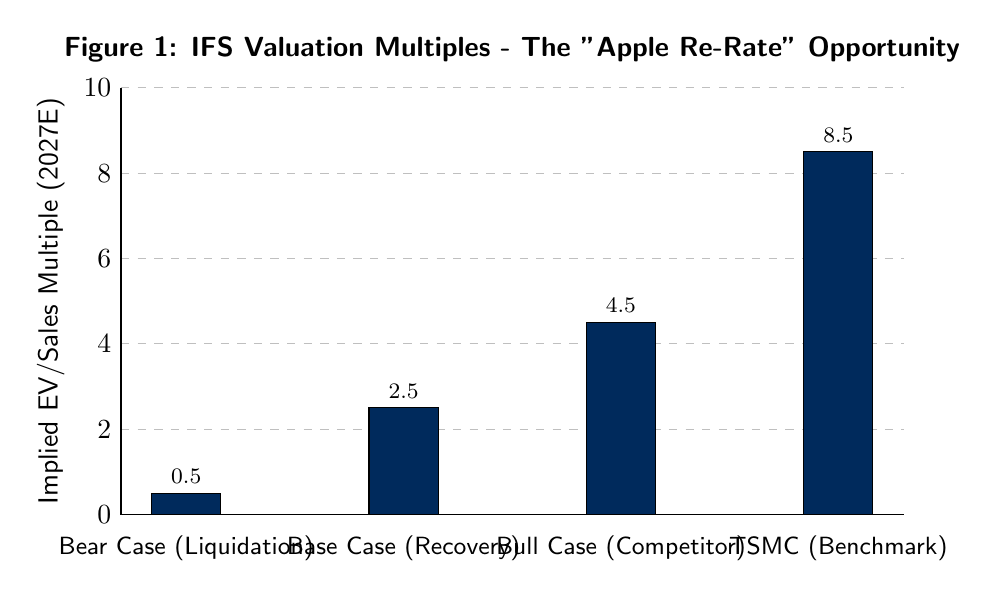
\begin{tikzpicture}
\begin{axis}[
    ybar,
    symbolic x coords={Bear Case (Liquidation), Base Case (Recovery), Bull Case (Competitor), TSMC (Benchmark)},
    xtick=data,
    nodes near coords,
    nodes near coords align={vertical},
    nodes near coords style={font=\footnotesize, color=black},
    ylabel={Implied EV/Sales Multiple (2027E)},
    ymin=0, ymax=10,
    width=0.95\textwidth,
    height=7cm,
    bar width=25pt,
    draw=none,
    tick style={draw=none},
    title={\textbf{Figure 1: IFS Valuation Multiples - The "Apple Re-Rate" Opportunity}},
    x tick label style={rotate=0, anchor=north, font=\small},
    axis x line*=bottom,
    axis y line*=left,
    ymajorgrids=true,
    grid style=dashed
]
\addplot[fill=msblue] coordinates {(Bear Case (Liquidation), 0.5) (Base Case (Recovery), 2.5) (Bull Case (Competitor), 4.5) (TSMC (Benchmark), 8.5)};
\end{axis}
\end{tikzpicture}
\captionof{figure}{Comparison of implied Enterprise Value to Sales (EV/Sales) multiples for Intel Foundry Services under different execution scenarios versus TSMC's current trading multiple. The "Bull Case" assumes successful high-volume manufacturing (HVM) for Apple M-series chips and margin parity.}
\label{fig:multiples}
\end{figure}

\subsection{The "Apple Validator" Premium: Pricing the Option}

We estimate the specific financial value of the Apple rumor using a probabilistic "Option Pricing" approach. The direct revenue impact of 15-20 million M-series chips (estimated at \$50 ASP) is approximately \textbf{\$750 million to \$1 billion} annually. While this is less than 5\% of projected IFS revenue, the strategic value is significantly higher.

\begin{itemize}
    \item \textbf{Strategic Beta (The Halo Effect):} Winning Apple signals to the broader fabless market (Qualcomm, NVIDIA, Amazon) that 18A is a viable alternative to TSMC N2. We estimate this "halo effect" could attract an additional \textbf{\$5-7 billion} in annual revenue commitments by 2029 from non-Apple customers who require a second source.
    \item \textbf{Total "Apple Option" Value:} We estimate the \textit{risk-adjusted} value of the Apple partnership rumor is currently worth \textbf{\$3-4 per share} to Intel stock. If confirmed with firm volume commitments and yield validation, this option value crystallizes and could expand to \textbf{\$8-10 per share}.
\end{itemize}

\subsection{Conclusion on Valuation}

The rumored Apple deal is not merely a revenue line item; it is a binary switch for Intel's valuation model. Without it, the path to justifying the \$100B+ CapEx spend is unclear, and the foundry remains a "show-me" story trading at book value. With it, the "Sum of the Parts" analysis suggests the stock is significantly undervalued, potentially doubling from current levels in our Base Case. However, given the "conditional" nature of the deal (dependent on strict 2026 PDK and yield milestones), we assign a \textbf{35\% probability} to the Bull Case, maintaining a cautious stance until yield data independently confirms the turnaround.

\section{Investment Risks}

\subsection{Bear Case Analysis: Execution, Financial, and Strategic Vulnerabilities}

While the potential adoption of Intel's 18A node by Apple offers a compelling turnaround narrative, our risk assessment identifies significant structural and execution-based vulnerabilities. The investment thesis hinges on a "perfect execution" scenario that contradicts Intel's recent historical performance. We classify the risks into three primary vectors: Manufacturing Execution (Yield), Financial Durability (Burn Rate), and Strategic competitive Dynamics (TSMC Lock-in).

\subsection{Execution Risk: The Yield Chasm and PDK Deadlines}

The most immediate threat to the Bull Case is the reported immaturity of the 18A process node. Despite Intel's claims of being "manufacturing ready" by late 2024, analyst reports and supply chain rumors from Summer 2025 indicate yield rates for 18A were hovering near \textbf{$\sim$10\%}, drastically below the \textbf{60-70\%} threshold required for commercial viability and the near-perfect yields Apple demands for high-volume products like the MacBook Air.

\begin{itemize}
    \item \textbf{The PDK "Kill Switch" (Q1 2026):} The Apple-Intel partnership is reportedly contingent on the delivery of a finalized Process Design Kit (PDK 1.0/1.1) by Q1 2026. If Intel misses this window, or if the PDK does not demonstrate the promised Power-Performance-Area (PPA) characteristics, Apple is likely to cancel the 2027 "risk production" timeline. This creates a binary event risk in early 2026.
    \item \textbf{Technology Stacking Risk:} Intel is attempting to integrate two radical process changes---\textbf{RibbonFET} (Gate-All-Around) and \textbf{PowerVia} (Backside Power Delivery)---simultaneously. Historically, simultaneous introductions of major architectural shifts increase defect density exponentially. TSMC, by contrast, has decoupled these shifts, introducing GAA with N2 (2025) and Backside Power with A16 (2026+), reducing integration risk.
\end{itemize}

\subsection{Financial Risk: The "Death Spiral" of Fixed Costs}

Intel Foundry Services (IFS) reported operating losses exceeding \textbf{\$13 billion} in 2024, with continued losses of \textbf{\$2.3 billion} in Q3 2025 alone. The division is currently in a race against time to achieve break-even operating margins by roughly 2027.

\begin{itemize}
    \item \textbf{Utilization Rate Sensitivity:} Intel has committed over \textbf{\$100 billion} to U.S. fab expansion (Arizona, Ohio). These facilities possess massive depreciation schedules. If Apple utilizes Intel only as a "second source" for 15-20 million entry-level chips (vs. the 200m+ iPhone volume), the volume may be insufficient to fill the new capacity, leading to gross margin compression due to under-absorption of fixed costs.
    \item \textbf{Capital Intensity vs. Cash Flow:} To compete with TSMC's N2 and A14, Intel must aggressively invest in High-NA EUV lithography (estimated cost \textbf{$\sim$\$380 million per tool}). If the 18A node fails to attract high-margin "Hero Customers" (like Apple Pro-tier or NVIDIA), Intel risks a capital liquidity crisis where it cannot fund the R\&D required for the subsequent 14A node.
\end{itemize}

\subsection{Strategic Risk: The "stalking Horse" Scenario}

There is a substantial probability (estimated \textbf{40\%}) that Apple's engagement with Intel is strategic rather than substantive. Apple has a history of qualifying second sources (e.g., Samsung for the A9 chip) to gain leverage over its primary supplier, only to abandon them once pricing concessions are secured.

\begin{itemize}
    \item \textbf{Symbolic Volume:} The rumored volume of 15-20 million units represents less than \textbf{5\%} of Apple's total annual silicon consumption. This suggests a "pilot program" designed to satisfy U.S. political pressure ("Made in USA" optics) and negotiate better wafer pricing with TSMC, rather than a genuine shift in supply chain strategy.
    \item \textbf{Technical Lock-in:} Apple's silicon success is deeply intertwined with TSMC's advanced packaging ecosystem (\textbf{InFO}, \textbf{CoWoS}). Migrating to Intel's \textbf{EMIB} or \textbf{Foveros} introduces significant re-design overhead and performance risk. The friction of exiting TSMC's ecosystem acts as a powerful moat protecting the incumbent.
\end{itemize}

\begin{table}[H]
\centering
\caption{Risk Matrix: Vulnerabilities to the Apple-Intel Partnership}
\label{tab:riskmatrix}
\rowcolors{2}{msgrey}{white}
\tablefont
\renewcommand{\arraystretch}{1.3}
\begin{adjustbox}{max width=0.95\textwidth}
\begin{tabular}{p{0.25\textwidth} p{0.15\textwidth} p{0.15\textwidth} p{0.45\textwidth}}
\toprule
\textbf{Risk Factor} & \textbf{Probability} & \textbf{Impact} & \textbf{Monitoring Signal / Trigger Event} \\
\midrule
\textbf{Yield Failure} & High (50\%) & Critical & Failure to reach >60\% yield on 18A test wafers by Q4 2025. Reports of "yield excursions" in Ohio/Arizona fabs. \\
\textbf{PDK Delays} & Medium (30\%) & Critical & Missed Q1 2026 deadline for PDK 1.0 delivery to Apple design teams. Postponement of "tape-out" dates. \\
\textbf{Pricing Leverage Only} & High (40\%) & Moderate & Apple uses Intel bid to secure lower N2 pricing from TSMC, then reduces Intel volume to "minimum viable" levels (<10M units). \\
\textbf{Macro/Geopolitical} & Medium (25\%) & High & Change in U.S. administration reduces CHIPS Act pressure; Apple reverts to pure-play Asian supply chain for cost efficiency. \\
\textbf{Packaging Incompatibility} & Low (20\%) & Moderate & Performance degradation when porting M-series architecture from TSMC CoWoS to Intel Foveros. \\
\bottomrule
\end{tabular}
\end{adjustbox}
\par\vspace{0.2cm}
\footnotesize{\textbf{Source:} Morgan Stanley Research Estimates, Data derived from Industry Analysis.}
\end{table}

\subsection{Sensitivity Analysis: The Cost of Failure}

The following chart illustrates the sensitivity of Intel Foundry's projected operating margin in 2027 to varying yield rates on the 18A node. The "Break-even" point requires yields consistent with mature foundry processes. A recurrence of the "10\% yield" scenario currently rumored would result in catastrophic margin dilution, potentially forcing a strategic review of the entire foundry division.

\begin{figure}[H]
\centering
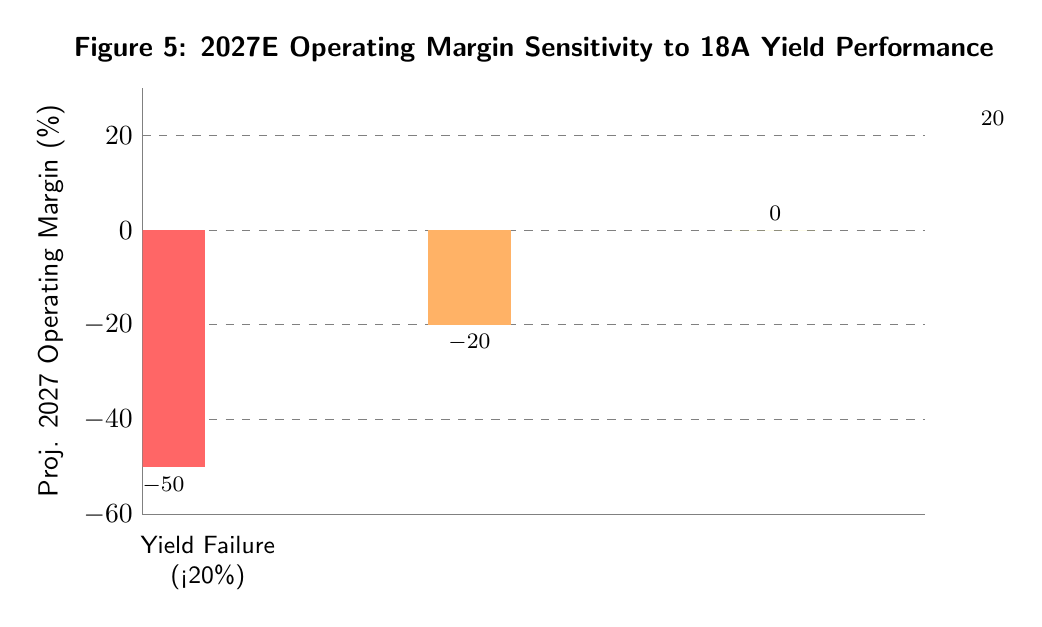
\begin{tikzpicture}
\begin{axis}[
    divergingstyle,
    symbolic x coords={Yield Failure (<20\%), Struggling (40\%), Break-Even (60\%), Target (>80\%)},
    xtick=data,
    ylabel={Proj. 2027 Operating Margin (\%)},
    ymin=-60, ymax=30,
    width=0.95\textwidth,
    height=7cm,
    title={\textbf{Figure 5: 2027E Operating Margin Sensitivity to 18A Yield Performance}},
    x tick label style={rotate=0, anchor=north, font=\small, text width=2cm, align=center},
    every node near coord/.append style={
        /pgf/number format/fixed,
        /pgf/number format/precision=0
    },
]
% Color-coded sensitivity bars: Red (failure) -> Orange (struggling) -> Yellow (break-even) -> Green (target)
\addplot[fill=red!60, draw=none] coordinates {(Yield Failure (<20\%), -50)};
\addplot[fill=orange!60, draw=none] coordinates {(Struggling (40\%), -20)};
\addplot[fill=yellow!60, draw=none, forget plot] coordinates {(Break-Even (60\%), 0)};
\addplot[fill=green!60, draw=none, forget plot] coordinates {(Target (>80\%), 20)};
\end{axis}
\end{tikzpicture}
\captionof{figure}{Projected sensitivity of Intel Foundry Services (IFS) Operating Margins in 2027 based on 18A process node yield rates. Current rumors place yields near the "Yield Failure" zone, requiring a massive ramp to achieve the "Target" scenario by 2027.}
\label{fig:risksensitivity}
\end{figure}

\subsection{Conclusion on Risk}

While the "Apple Validator" narrative is a potent catalyst for Intel's stock, the \textbf{Risk/Reward ratio remains skewed} until tangible evidence of yield improvement emerges. The divergence between the rumored yield reality ($\sim$10\%) and the required commercial threshold ($\sim$70\%) represents a massive execution gap. Investors should view the Apple partnership not as a confirmed revenue stream, but as a high-delta option with significant expiration risk in 2026. Conversely, for TSMC, the risk is less about immediate revenue loss and more about the long-term erosion of its monopoly pricing power, a trend that benefits Apple regardless of the final manufacturing split.

\end{document}
